%% This file was auto-generated by IPython.
%% Conversion from the original notebook file:
%% 125_years_of_data.ipynb
%%
%%\documentclass[11pt,english]{article}

%% This is the automatic preamble used by IPython.  Note that it does *not*
%% include a documentclass declaration, that is added at runtime to the overall
%% document.
\documentclass[conference,a4paper,twoside]{IEEEtran}
\usepackage{enumitem}
\usepackage{pgf}
\usepackage{tikz}
%\usepackage{graphicx}
%\usepackage{datatool}
%\usepackage{dataplot}
%\usepackage{xcolor}
\usetikzlibrary{calc,through,decorations.pathmorphing}
\usetikzlibrary{decorations.pathreplacing}
\usetikzlibrary{decorations.text}
%\usetikzlibrary{trees}
\usetikzlibrary{fit}
\usetikzlibrary{backgrounds}
\usetikzlibrary{positioning}
\usetikzlibrary{shapes,arrows}
\usetikzlibrary{shadows}
%\usetikzlibrary{calendar}
%\usepackage{array}
%\usepackage{ctable}
%\usepackage{dcolumn}
%\usepackage{mdwmath}
\usepackage{mdwtab}
\usepackage{setspace}
\usepackage{fancyhdr}
%\usepackage{amsmath}
\usepackage{url}
%Get rid of the paragraph indents...
\setlength{\parindent}{0mm}
\setlength{\textheight}{260mm}
% needed for markdown enumerations to work
\usepackage{enumerate}

% Slightly bigger margins than the latex defaults
%\usepackage{geometry}
%\geometry{verbose,tmargin=3cm,bmargin=3cm,lmargin=2.5cm,rmargin=2.5cm}

% Define a few colors for use in code, links and cell shading
\usepackage{color}
\definecolor{orange}{cmyk}{0,0.4,0.8,0.2}
\definecolor{darkorange}{rgb}{.71,0.21,0.01}
\definecolor{darkgreen}{rgb}{.12,.54,.11}
\definecolor{myteal}{rgb}{.26, .44, .56}
\definecolor{gray}{gray}{0.45}
\definecolor{lightgray}{gray}{.95}
\definecolor{mediumgray}{gray}{.8}
\definecolor{inputbackground}{rgb}{.95, .95, .85}
\definecolor{outputbackground}{rgb}{.95, .95, .95}
\definecolor{traceback}{rgb}{1, .95, .95}

% Framed environments for code cells (inputs, outputs, errors, ...).  The
% various uses of \unskip (or not) at the end were fine-tuned by hand, so don't
% randomly change them unless you're sure of the effect it will have.
\usepackage{framed}

% remove extraneous vertical space in boxes
\setlength\fboxsep{0pt}

% codecell is the whole input+output set of blocks that a Code cell can
% generate.

% TODO: unfortunately, it seems that using a framed codecell environment breaks
% the ability of the frames inside of it to be broken across pages.  This
% causes at least the problem of having lots of empty space at the bottom of
% pages as new frames are moved to the next page, and if a single frame is too
% long to fit on a page, will completely stop latex from compiling the
% document.  So unless we figure out a solution to this, we'll have to instead
% leave the codecell env. as empty.  I'm keeping the original codecell
% definition here (a thin vertical bar) for reference, in case we find a
% solution to the page break issue.

%% \newenvironment{codecell}{%
%%     \def\FrameCommand{\color{mediumgray} \vrule width 1pt \hspace{5pt}}%
%%    \MakeFramed{\vspace{-0.5em}}}
%%  {\unskip\endMakeFramed}

% For now, make this a no-op...
\newenvironment{codecell}{}

 \newenvironment{codeinput}{%
   \def\FrameCommand{\colorbox{inputbackground}}%
   \MakeFramed{\advance\hsize-\width \FrameRestore}}
 {\unskip\endMakeFramed}

\newenvironment{codeoutput}{%
   \def\FrameCommand{\colorbox{outputbackground}}%
   \vspace{-1.4em}
   \MakeFramed{\advance\hsize-\width \FrameRestore}}
 {\unskip\medskip\endMakeFramed}

\newenvironment{traceback}{%
   \def\FrameCommand{\colorbox{traceback}}%
   \MakeFramed{\advance\hsize-\width \FrameRestore}}
 {\endMakeFramed}

% Use and configure listings package for nicely formatted code
\usepackage{listingsutf8}
\lstset{
  language=python,
  inputencoding=utf8x,
  extendedchars=\true,
  aboveskip=\smallskipamount,
  belowskip=\smallskipamount,
  xleftmargin=2mm,
  breaklines=true,
  basicstyle=\small \ttfamily,
  showstringspaces=false,
  keywordstyle=\color{blue}\bfseries,
  commentstyle=\color{myteal},
  stringstyle=\color{darkgreen},
  identifierstyle=\color{darkorange},
  columns=fullflexible,  % tighter character kerning, like verb
}

% The hyperref package gives us a pdf with properly built
% internal navigation ('pdf bookmarks' for the table of contents,
% internal cross-reference links, web links for URLs, etc.)
\usepackage{hyperref}
\hypersetup{
  breaklinks=true,  % so long urls are correctly broken across lines
  colorlinks=true,
  urlcolor=blue,
  linkcolor=darkorange,
  citecolor=darkgreen,
  }

% hardcode size of all verbatim environments to be a bit smaller
\makeatletter 
\g@addto@macro\@verbatim\tiny\topsep=0.5em\partopsep=0pt
\makeatother 

% Prevent overflowing lines due to urls and other hard-to-break entities.
\sloppy




\begin{document}


% paper title
% can use linebreaks \\ within to get better formatting as desired
\title{125 years of data \\ \vspace{5mm} \large{EEA Conference 2013} \\ \normalsize{SKYCITY Convention Centre, Auckland, New Zealand, 19--21 June 2012}}

%Paper by: Friday 19th April, 2013;
% author names and affiliations
% use a multiple column layout for up to three different
% affiliations
%\author{\IEEEauthorblockN{\Large David Hume, \normalsize BE, PhD, MIEEE, MIET}
%\IEEEauthorblockA{Electricity Authority \\
%\emph{Email: david.hume@ea.govt.nz}}}
\author{\IEEEauthorblockN{David Hume}
\IEEEauthorblockA{Electricity Authority, Level 7, 2 Hunter Street, Wellington \\  
Email: david.hume@ea.govt.nz} } 

% make the title area

\maketitle
\thispagestyle{plain}
\pagestyle{plain}

%\fancyfoot[CE,CO]{\footnotesize \thepage\ of \pageref{LastPage}}
%\fancyfoot[LE,LO]{\footnotesize 125 years of data}

\IEEEpeerreviewmaketitle


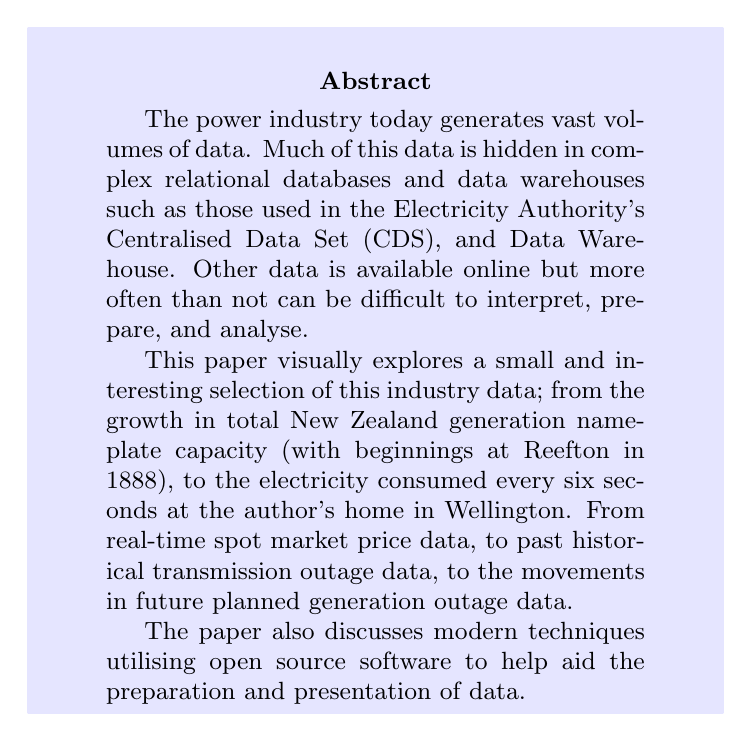
\begin{tikzpicture}
\draw (50,0) node[top color=blue!10,text width=8.6cm,text justified, bottom color=blue!10]
{
\begin{abstract}
\setstretch{0.99}
\normalfont\small

The power industry today generates vast volumes of data. Much of this data is hidden in complex relational databases and data warehouses such as those used in the Electricity Authority's Centralised Data Set (CDS), and Data Warehouse. Other data is available online but more often than not can be difficult to interpret, prepare, and analyse.

This paper visually explores a small and interesting selection of this industry data; from the growth in total New Zealand generation nameplate capacity (with beginnings at Reefton in 1888), to the electricity consumed every six seconds at the author's home in Wellington. From real-time spot market price data, to past historical transmission outage data, to the movements in future planned generation outage data.

The paper also discusses modern techniques utilising open source software to help aid the preparation and presentation of data.


\end{abstract}

%\begin{keywords}

%\end{keywords}

};

\end{tikzpicture}

\section{Introduction}
\setstretch{1}

This paper provides results and analysis from a smorgasbord of data-series within the NZ electrical power system.  Most of this data is either openly available on-line, or through the Centralised Data Set (CDS).  

Data analysis often requires significant time and effort wrangling (or munging) the data into a required form suitable for analysis and then visualisation.  The output of this work, often a shared visualisation, can lead to further feedback and questions like, why? and how? which can lead to yet further analysis and updated visualisation.  Although this process is often rewarding, it can take significant time and effort with out the appropriate tools.  The authors tools of choice, all open source and freely available, include: Python and the ``iPython notebook'', plus the Pandas,NumPy and Matplotlib python modules, among many others.  

\begin{figure*}[hbtm]
\begin{center}
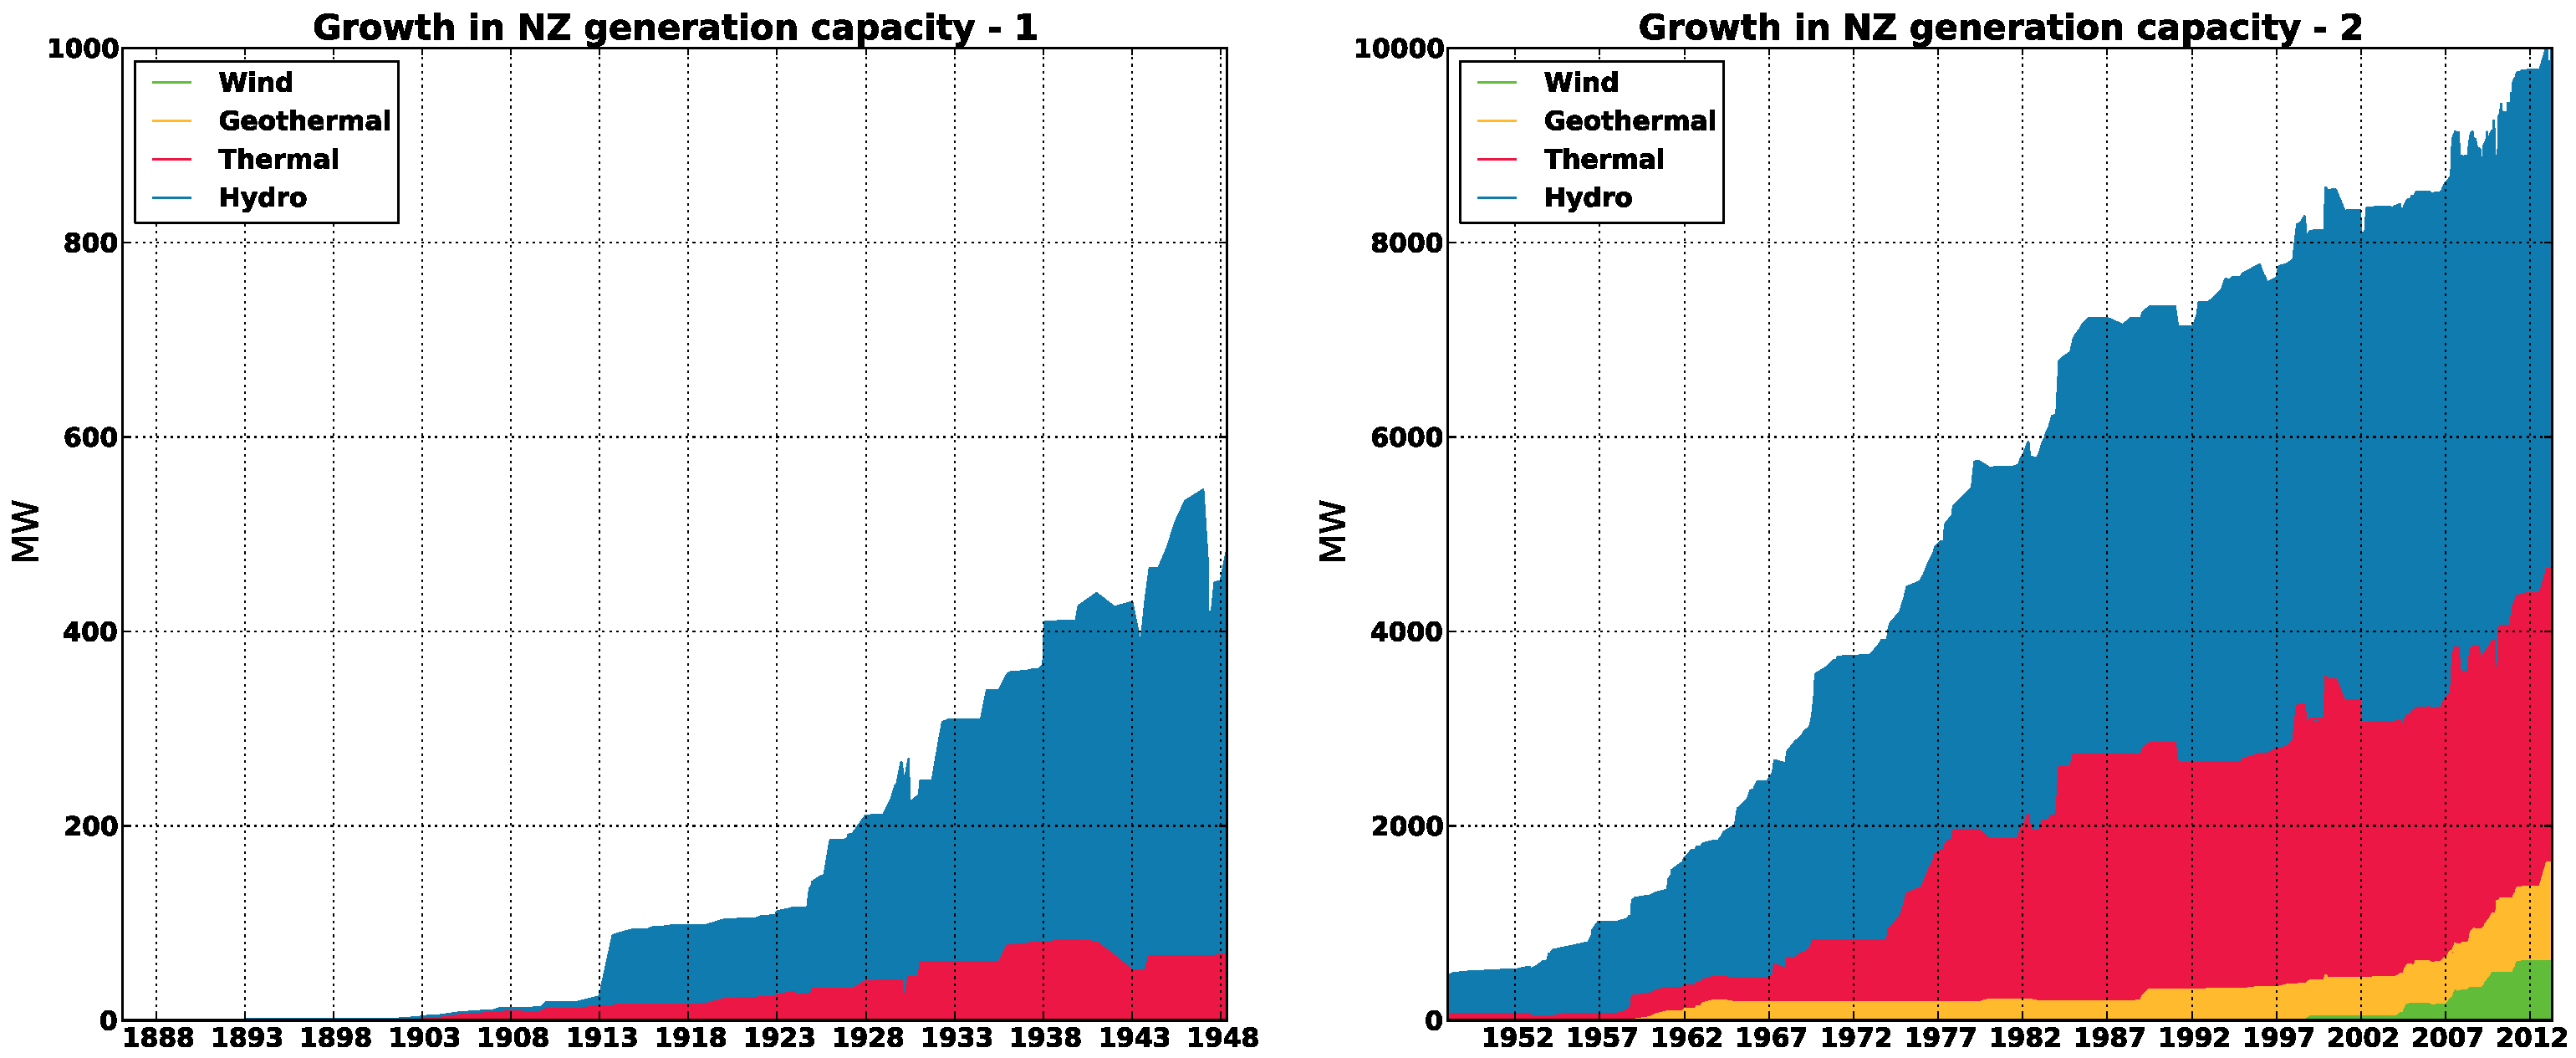
\includegraphics[width=1\textwidth]
{125_years_of_data_files/125_years_of_data_fig_00.pdf}
\par
\end{center}
\end{figure*}

In line with this years conference theme, Section~\ref{sec:np} presents a very small data set representing the growth of name-plate generation capacity in New Zealand.  This series begins, not 125 years ago at Reefton, but 127 years ago at a private gold field near Queenstown.

%Recorded every 6 seconds to a database running on a Raspberry Pi computer, this data represents, perhaps, a small part of what future ``Big Data'' may look like on the demand side of the industry.  

Jumping ahead to today, Section~\ref{sec:rp} investigates the electrical demand of the authors Wellington home while Section~\ref{sec:5m}, explores a small sample set of energy price data including real-time 5 minute prices.

Using data published in the Centralised Data Set, Section~\ref{sec:fo} explores, and attempts to identify any trends present in forced transmission outage data while Section~\ref{sec:po} briefly explores the Planned Outage Co-Ordination Process (or POCP).  This database, run by the System Operator, is used by Transpower (as asset owner), 
and most Generators to publicise planned outages.  Finally, Section~\ref{sec:os} provides a brief over-view of the open source software used by the author for all analysis and presentation used in this paper.

\section{Growth in New Zealand generation capacity}\label{sec:np}

%Interesting links 

%<p>Bullendale links
%http://www.doc.govt.nz/Documents/science-and-technical/sap237.pdf
%http://www.doc.govt.nz/Documents/science-and-technical/sap237b.pdf
%http://www.doc.govt.nz/Documents/science-and-technical/sap237c.pdf
%Reefton links
%http://www.reefcottage.co.nz/41_history.htm   
%http://www.reeftongold.co.nz/morning-heritage-tours/electric-light
%http://www.TeAra.govt.nz/en/gold-and-gold-mining/12/2
%
%\emph{\ldots On Wednesday the 24'th of November 1886, bright light had been brought to the bars of Dawson's, Kater's, Stevenson's and William's hotels by showman Walter Prince via underground cable through attaching a one kilowatt generator to the Oxley's brewery's steam engine. The test required regular visits of the spectators between the hotel and the brewery, and there was high demand at each point of supply. As a result, many were carrying an overload and it was not only the hotel that was lit up.\ldots''}
%\begin{flushright}
%\small Electricity Development in New Zealand.
%\end{flushright}
%On Monday the 6'th of December the Reefton Electrical Transmission of Power and Lighting company was formed with Mr. Prince as a major shareholder, to construct a hydro power station on the far bank of the Inangahua river. From an intake opposite Black's Point on the Inangahua river, a canal and two short tunnels (passing a slip and the main bluff) enabled a head of 27 feet to supply a 70 horsepower Rafel water turbine built in Dunedin that was connected by belt to a Crompton DC dynamo generating 20KW (=27HP) at 30 and 110 volts, sufficient for five hundred lights. The water races were ready by February, but there were delays in the arrival of the machines and the lamps.

%The power station made its first demonstration shortly after seven p.m. on Wednesday 1'st August 1888 when an arc light lit "the whole scene with strange but dazzling brilliance" (Inangahua Times). Aerial conductors conveyed power across the river to Oddfellows Hall where on Saturday the 4'th of August there was a second demonstration of fifty incandescent filament lamps, giving a much more pleasant light than the arc lamp. By September, some 130 lamps were being served, but insulation problems with the underground cables from the Odfellows Hall supply point caused intermittent service that Mr. Prince was unable to correct. The Telegraph Department had required underground lines to avoid risk to its overhead telegraph lines. Mr. J.J. Horton was hired in his place and and on arriving on the thirteenth of October found that the wiring was of different gauges, badly jointed and insulated. By Christmas some 500 lights were being supplied.

%This was New Zealand's first electricity generator for public use, being street lights, then home lights. The rate in 1888 from the Reefton Electrical Transmission of Power and Lighting Company, Ltd. was three pounds per light per year, used or not. The connection cost was one pound, paid once only. A good salary at the time was a hundred pounds a year. The sixteen candlepower lamps were made in London and cost one shilling and three pence each.

%A second public trail of the electric light system was made on Saturday evening last in Broadway. The night was fortunately very favorable for the display, and an immense crowd of people gathered in the street to witness the exhibition, and when, shortly before 8 p.m., 
\emph{\ldots the powerful light of the arc-lamp burst forth, like a flash of a mighty meteor, a murmur of admiration rose from the spectators, and there was an immediate scampering of feet towards the screen of the display. As on the former occasion, the light throbbed a good deal, but at its maximum brilliancy illuminated the town over a very wide area, with its cold, cheerless, phosphorescent rays\ldots
%The illumination reached far upon the mountains round the town, and gave a very sepulchral appearance to the hill-sides, the trees and stumps standing out in the strange pallid light, like so may tombstones. 
But if the arc-light was an attraction outside, the interior of the Oddfello's Hall was infinitely more so. Rows of lamps were suspended from the building, encased in a variety of fantastically shaped shades of different colours, and the whole scene was one of stricken splendour. It was indeed a ``Hall of dazzling light\ldots''}
\begin{flushright}
\small Inangahua Herald, 6/9/1888

\end{flushright}
 
Over the last several years Nicky McLean from the Electricity Authority has put together a very small, but interesting historical record of electricity generation in New Zealand.  The series, though continually being updated is enough to provide a good indication of the growth in generation capacity in New Zealand over the last 127 years.

The data includes; estimated nameplate capacity, approximate commissioning and decommissioning dates as well as useful comments. Sometimes a start date has a precision down to the hour, at other times it is down to just the year (in which case it is assumed to be commissioned/decommissioned at the beginning of the year).  %When generation is known to have an end date, or has been temporary decommissioned, a negative of the nameplate value is used, allowing a computer program to correctly sum up total nameplate capacity over time.
    
The raw data file used in this paper is publically available as a simple text file and provided as part of the Centralised Data Set (CDS).   As some care has been taken over the format of the file, it is able to be read (parsed) with a simple computer program.  In this case, a small Python script has been used to parse the data into memory from where the data can then be examined for further analysis and visualisation (see Figure~\ref{fig:npg}). 

We see that perhaps the first recorded use of electricity in New Zealand was 127 years ago on the 3rd of February, 1886, at the private Bullendale gold mine (two years before the public power supply started at Reefton).  Interestingly, the Bullendale scheme was DC and included New Zealand's first DC transmission link from the power house to where the power was required at a nearby quartz stamping battery.   Two years later, on the 1st of August, 1888, Reefton demonstated the first public supply of electricity in New Zealand.  The rest, as they say, is history\ldots\footnote{Additional historical events will be talked about in the presentation.} 
\vspace{3mm}

\emph{`Very little is yet really known about electricity'}
\begin{flushright}
\small Mines Inspector commenting on the new \\ electric dynamos at the Bullendale, 1887. 
\end{flushright}


\begin{figure*}[hbtm]
\begin{center}
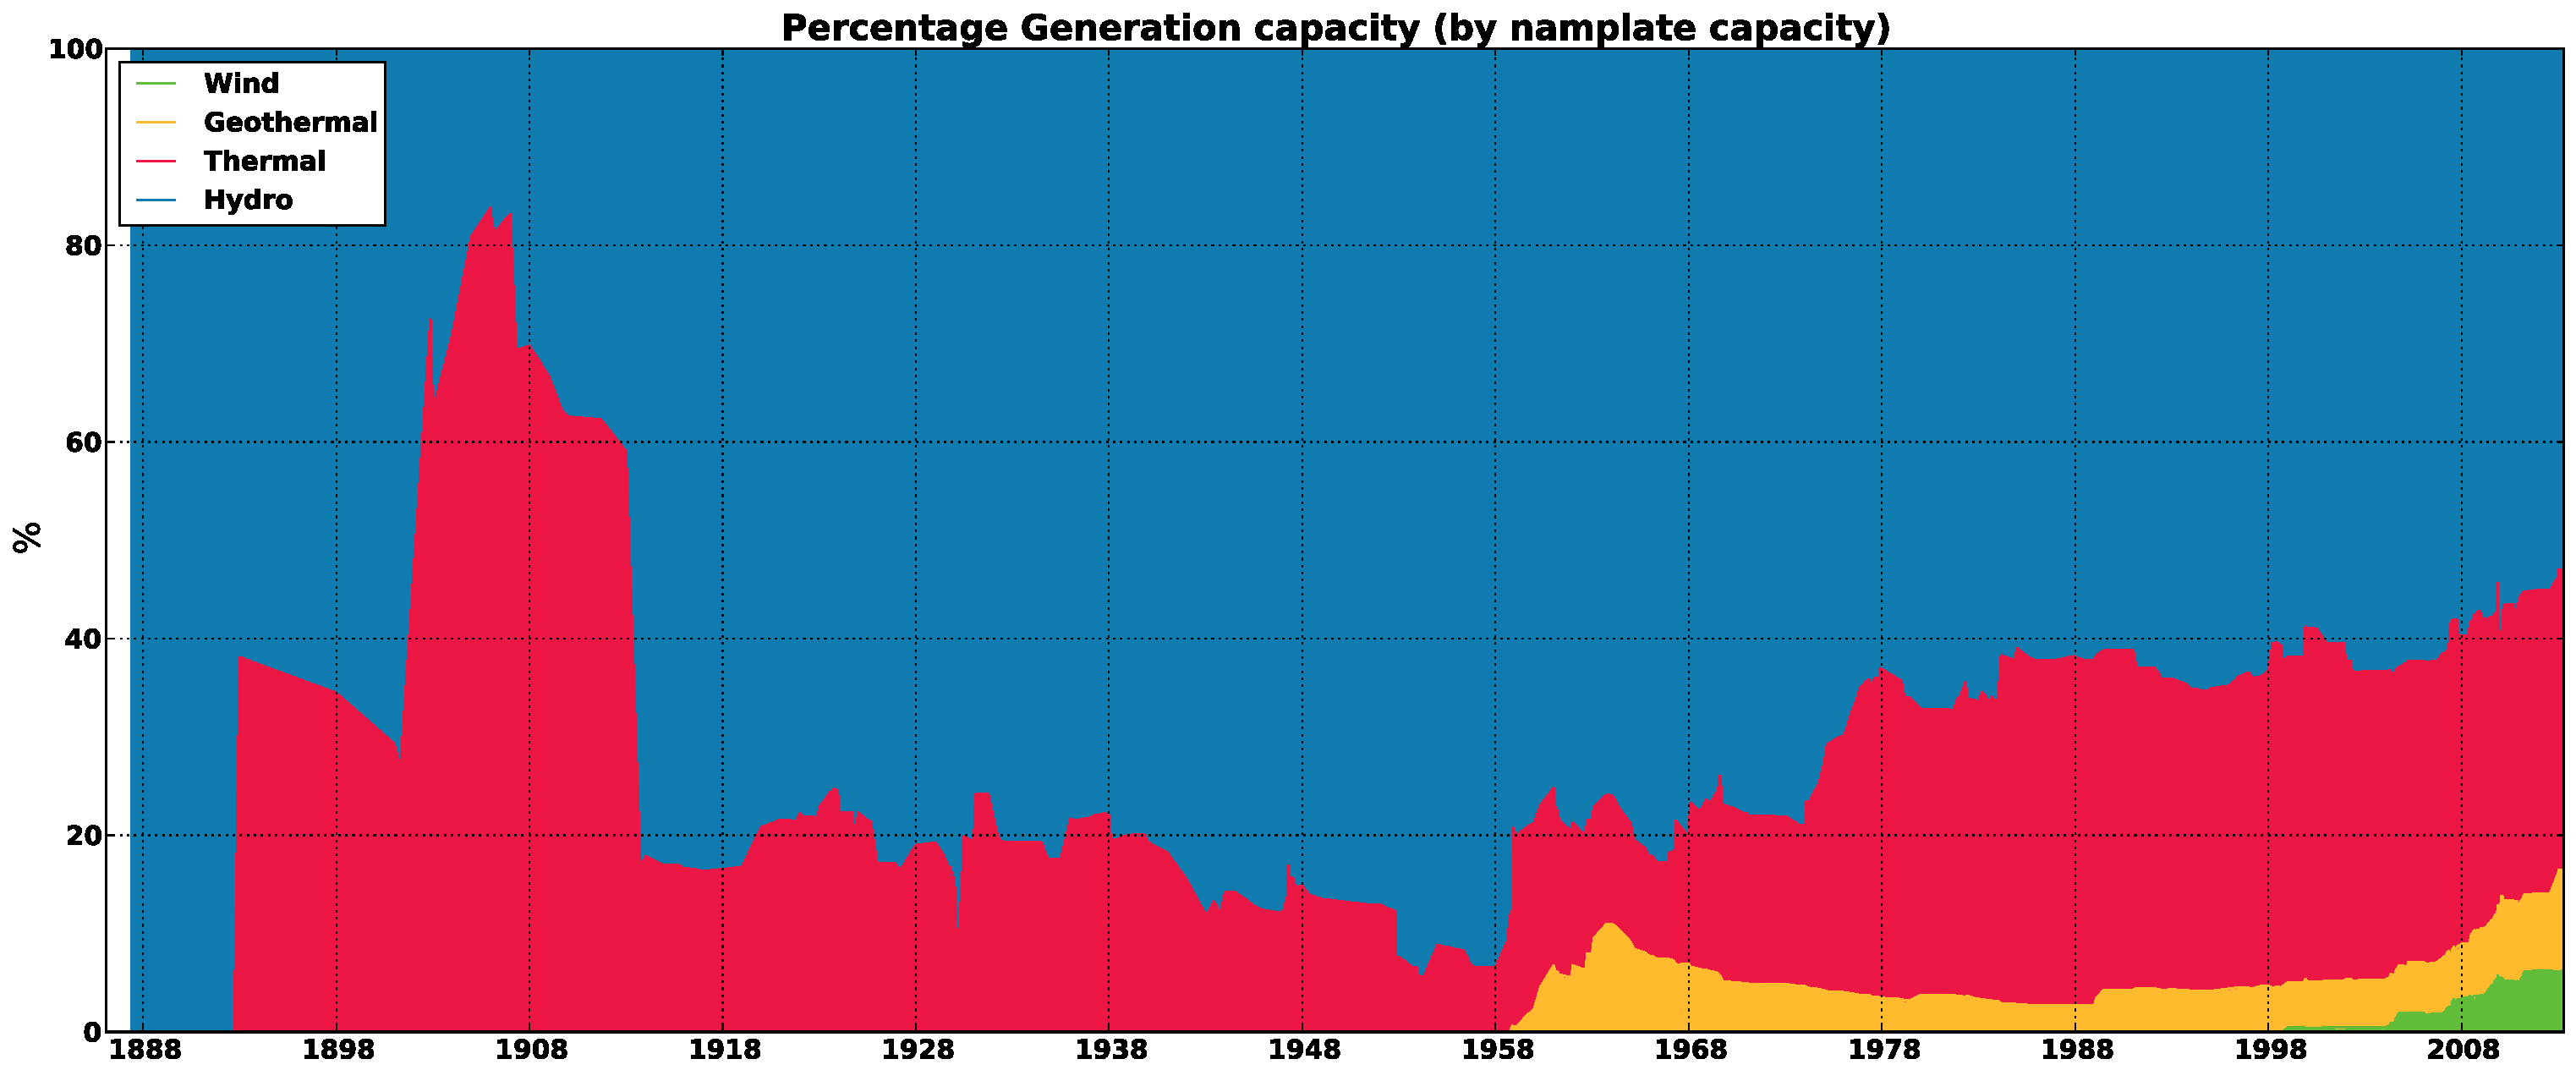
\includegraphics[width=1\textwidth]{125_years_of_data_files/125_years_of_data_fig_02.pdf}
\par
\end{center}
\caption{125 years of data illustrating the approximate historical generation capacity growth in New Zealand.}
\label{fig:npg}
\end{figure*}

\newpage
%http://en.wikipedia.org/wiki/Horahora_Power_Station    
\section{Home energy monitoring}\label{sec:rp}
\setstretch{0.95}
In complete contrast to the previous section we jump 127 years to the present day and the data, collected at the authors home, of total house-hold electrical consumption.  At the time of writing, ~5 months of data has been recorded at a 6 second resolution into a database containing over 1.7 million rows, and growing.  This is a single reading for a single household.  The increase of smart meters in New Zealand means many similar datasets could exist\footnote{Perhaps not at this resolution?}.   Through analysis of the data, owners (of the data) could benefit from its use.  For example, one could imagine a future where individual house-hold data could be used to help tailor individual customer tariff plans?, or, help retailers target suitable customers for their portfolio?\footnote{Perhaps this is already happening to some extent?}

Even without a smart meter, it is relatively straight-forward (with the aid of various internet blogs) for an electrical engineer to set up a low cost house-hold energy monitoring system.  

The system described here consists of:
\begin{enumerate}
\item a Raspberry Pi computer; and, 
\item an off-the-shelf energy monitoring kit (Current Cost + USB data cable).
\end{enumerate}
    
Every 6 seconds the Current Cost logs the energy use at the mains switch-board of the authors home.  This is recorded to a MySQL database running on the Raspberry Pi, from which the data can be downloaded and then analysed. 

Figure~\ref{fig:hm} illustrates a typical high-usage day.  The house-hold consists of two adults, and two young children and so should represent the energy usage of a typical young family living in New Zealand.  Other characteristics of the house-hold include:
\begin{enumerate}
\item electric hot water;
\item solid fuel (wood) burner; 
\item electric oven; 
\item gas hob; 
\item one fridge-freezer and one small chest freezer; 
\item house is located in Wellington, over 200m above sea-level.
\end{enumerate}

\setstretch{0.95}

%\begin{figure*}[hbtm]
%\begin{center}
%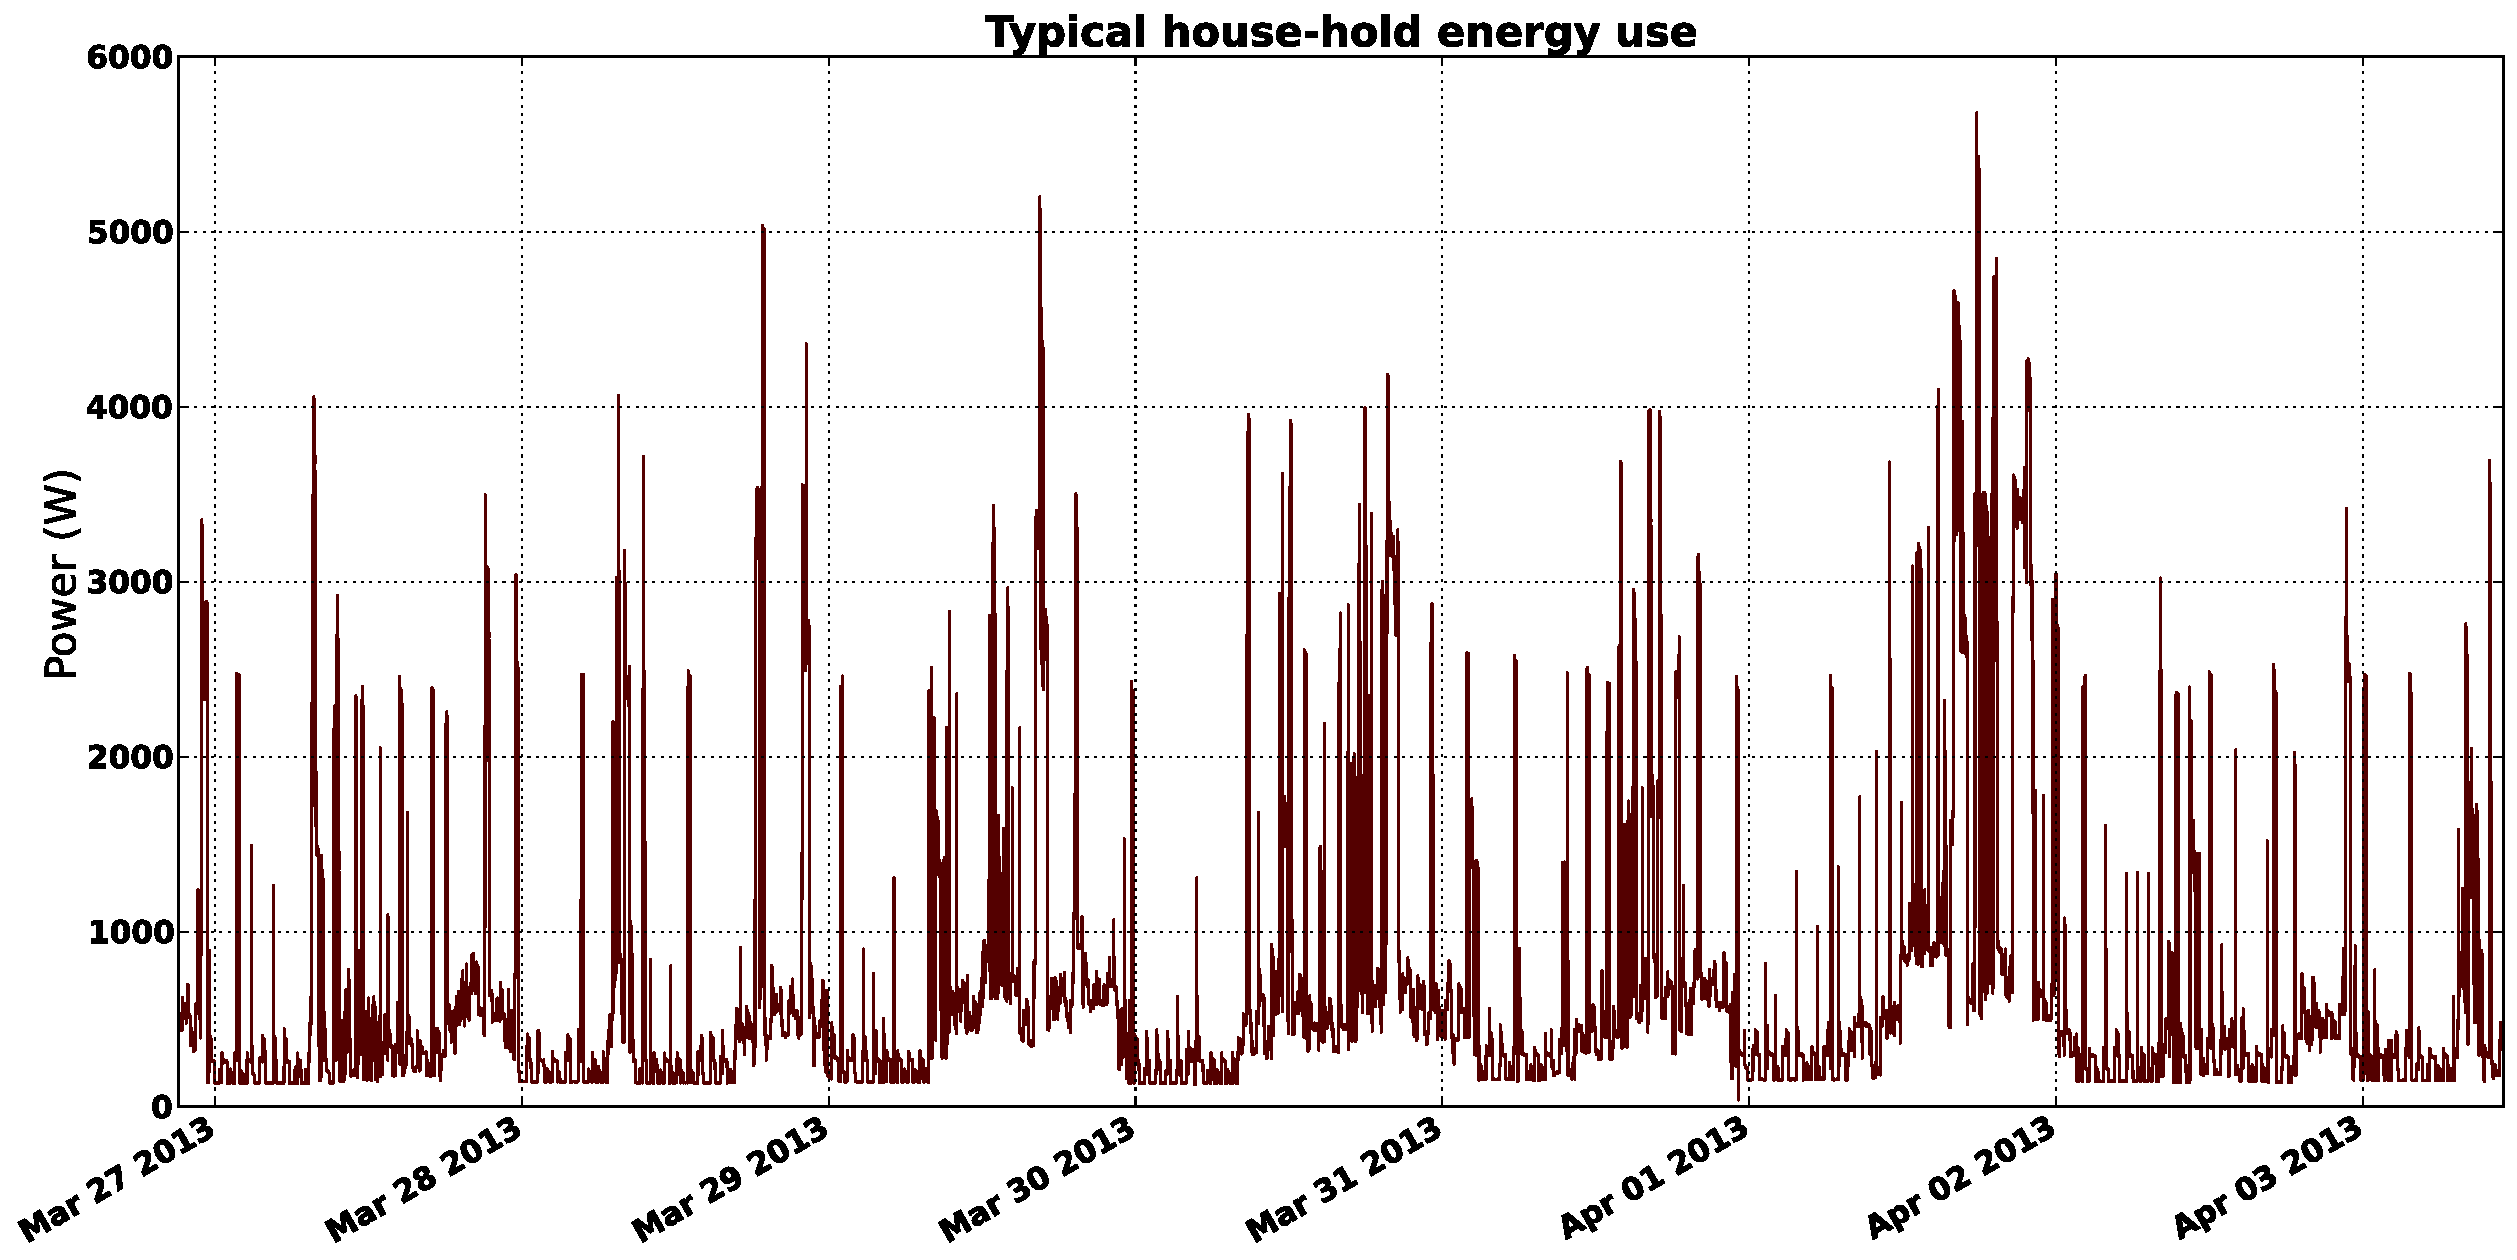
\includegraphics[width=1\textwidth]{125_years_of_data_files/125_years_of_data_fig_03.pdf}
%\par
%\end{center}
%\end{figure*}

\begin{figure*}[hbtm]
\begin{center}
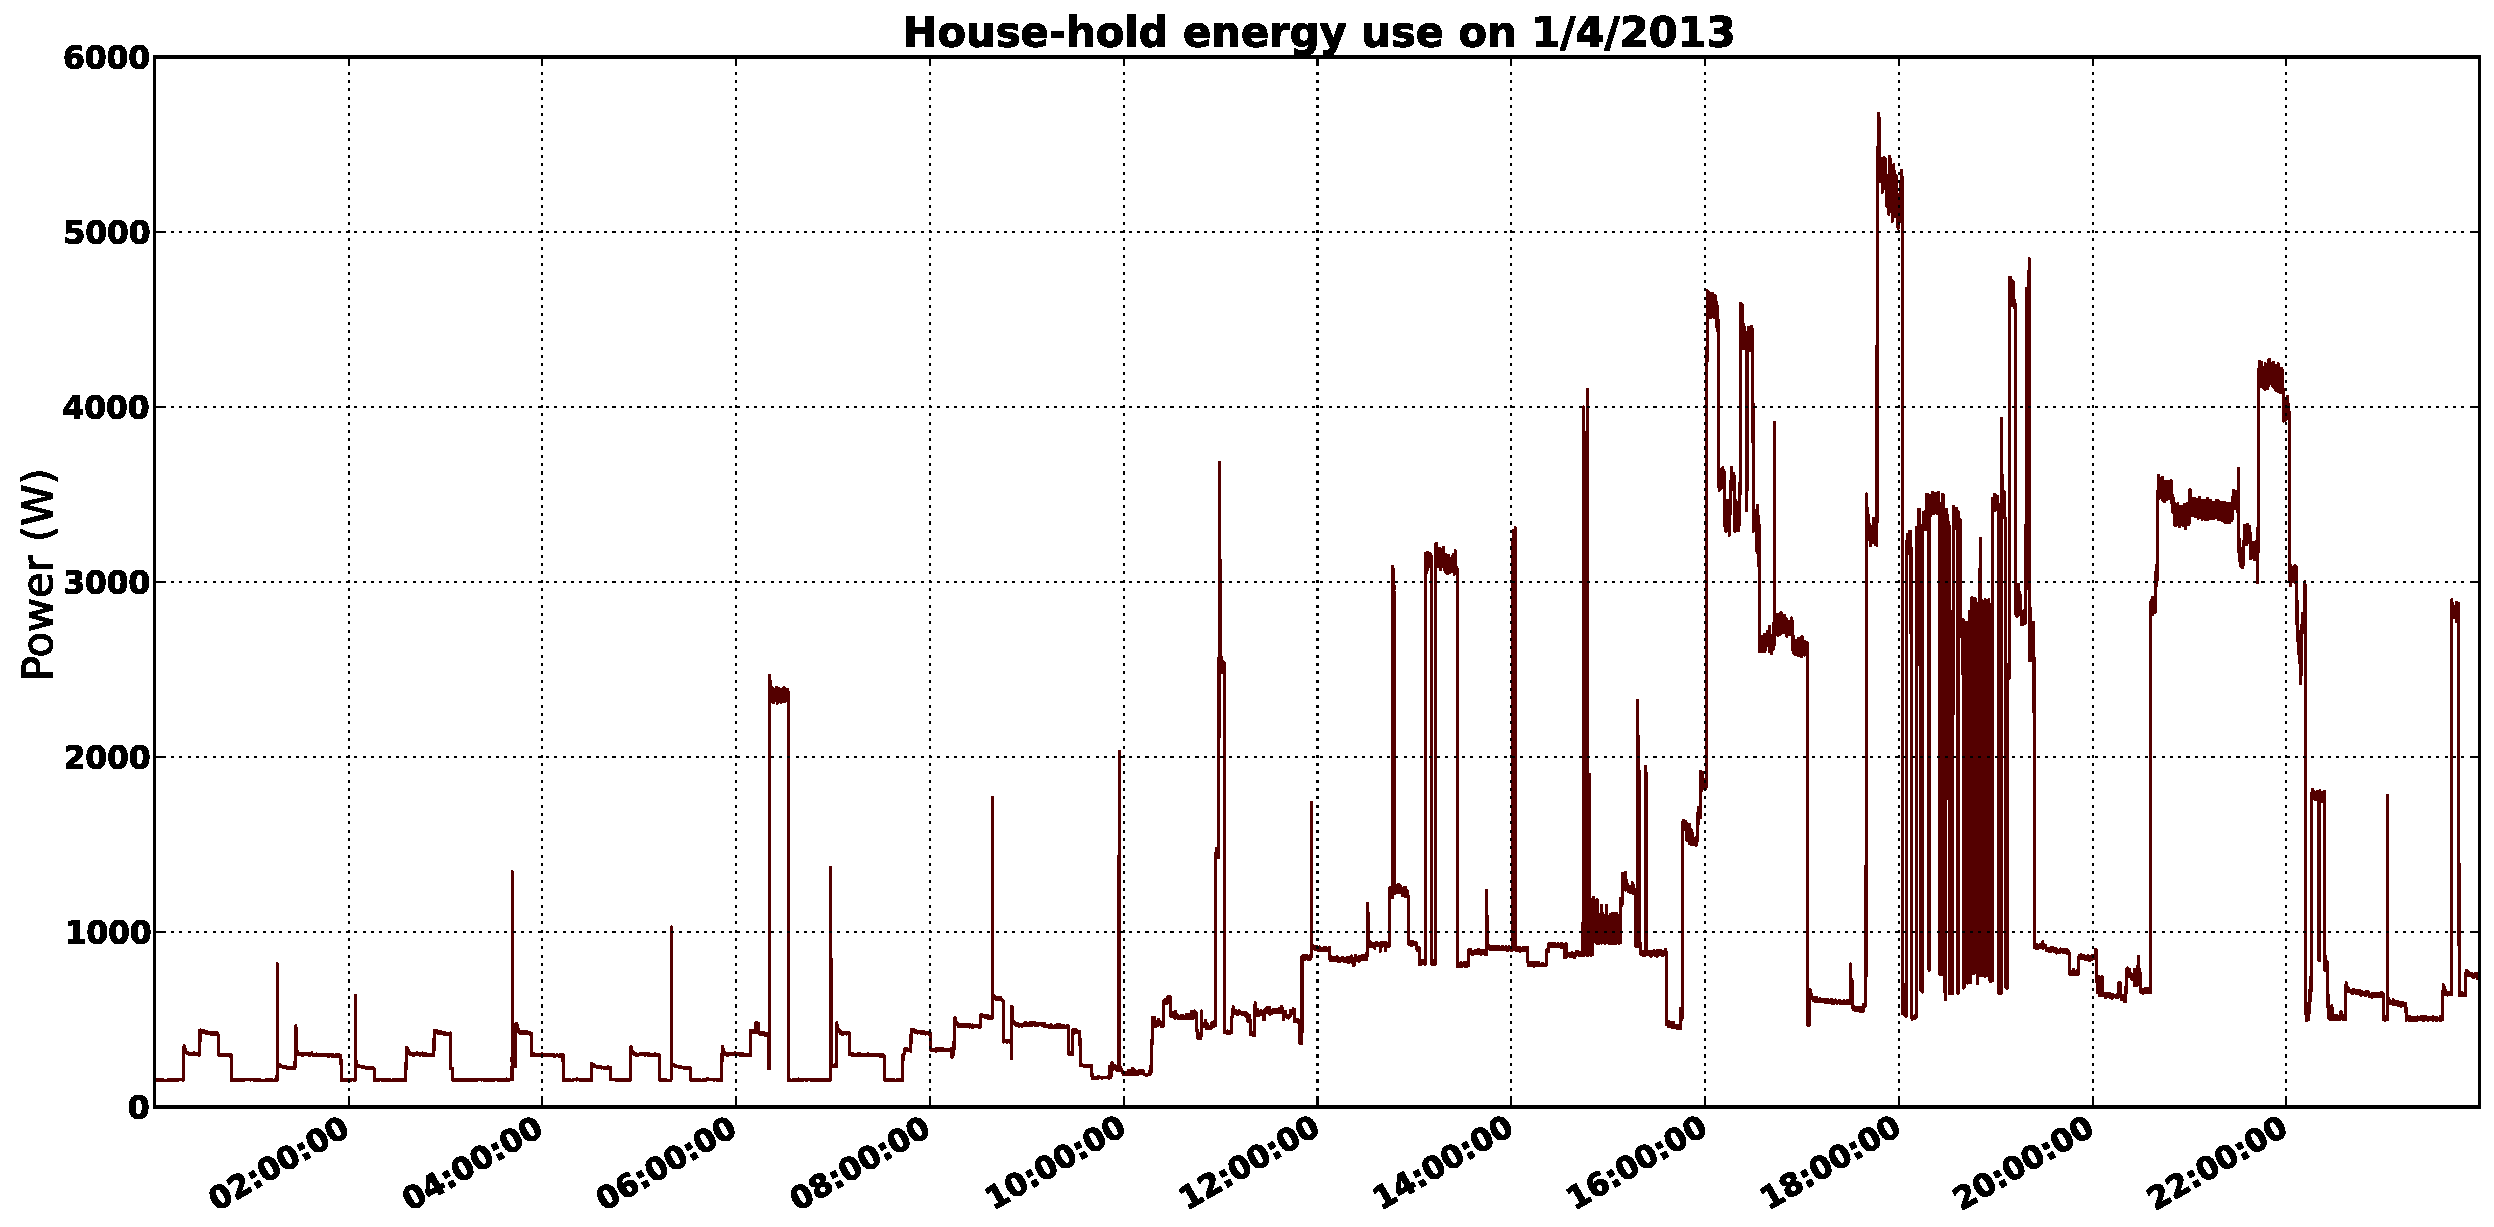
\includegraphics[width=1\textwidth]{125_years_of_data_files/125_years_of_data_fig_04.pdf}
\par
\end{center}
\caption{Typical house-hold electrical energy use.}
\label{fig:hm}
\end{figure*}

In several instances the inductive inrush current of the fridge and freezer can be observed as a clear spike.  In the act of observing such time series data, one can start to identify different appliance loads by eye!  For example, on this particular day the washing machine was switched on just prior to the 3pm School pickup, the kids had a bath before dinner and the oven was turned on just prior to 6pm, from memory, to cook a delicious quiche! 

In terms of the demand profile, it is interesting to observe how our demand compares with the average demand for our region.  This sort of analysis could help retailers in the future profile customers demand patterns.  Figure~\ref{fig:dp} illustrates the mean daily profile of the authors home, compared with the mean daily profile of the closest GXP (Wilton 33kV) which supplies the region. 

One could deduce from this that the occupants of this home tend to sleep in!  The morning peak electricity usage has a clear lag of $\approx$1 hour compared with the regional demand.  Additionally, there is a clear after school/dinner peak.   The author is a little unclear of the cause of the bump at 10pm. This may be caused by hot-water and running the dishwasher.  
\begin{figure}[hbtm]

\begin{center}
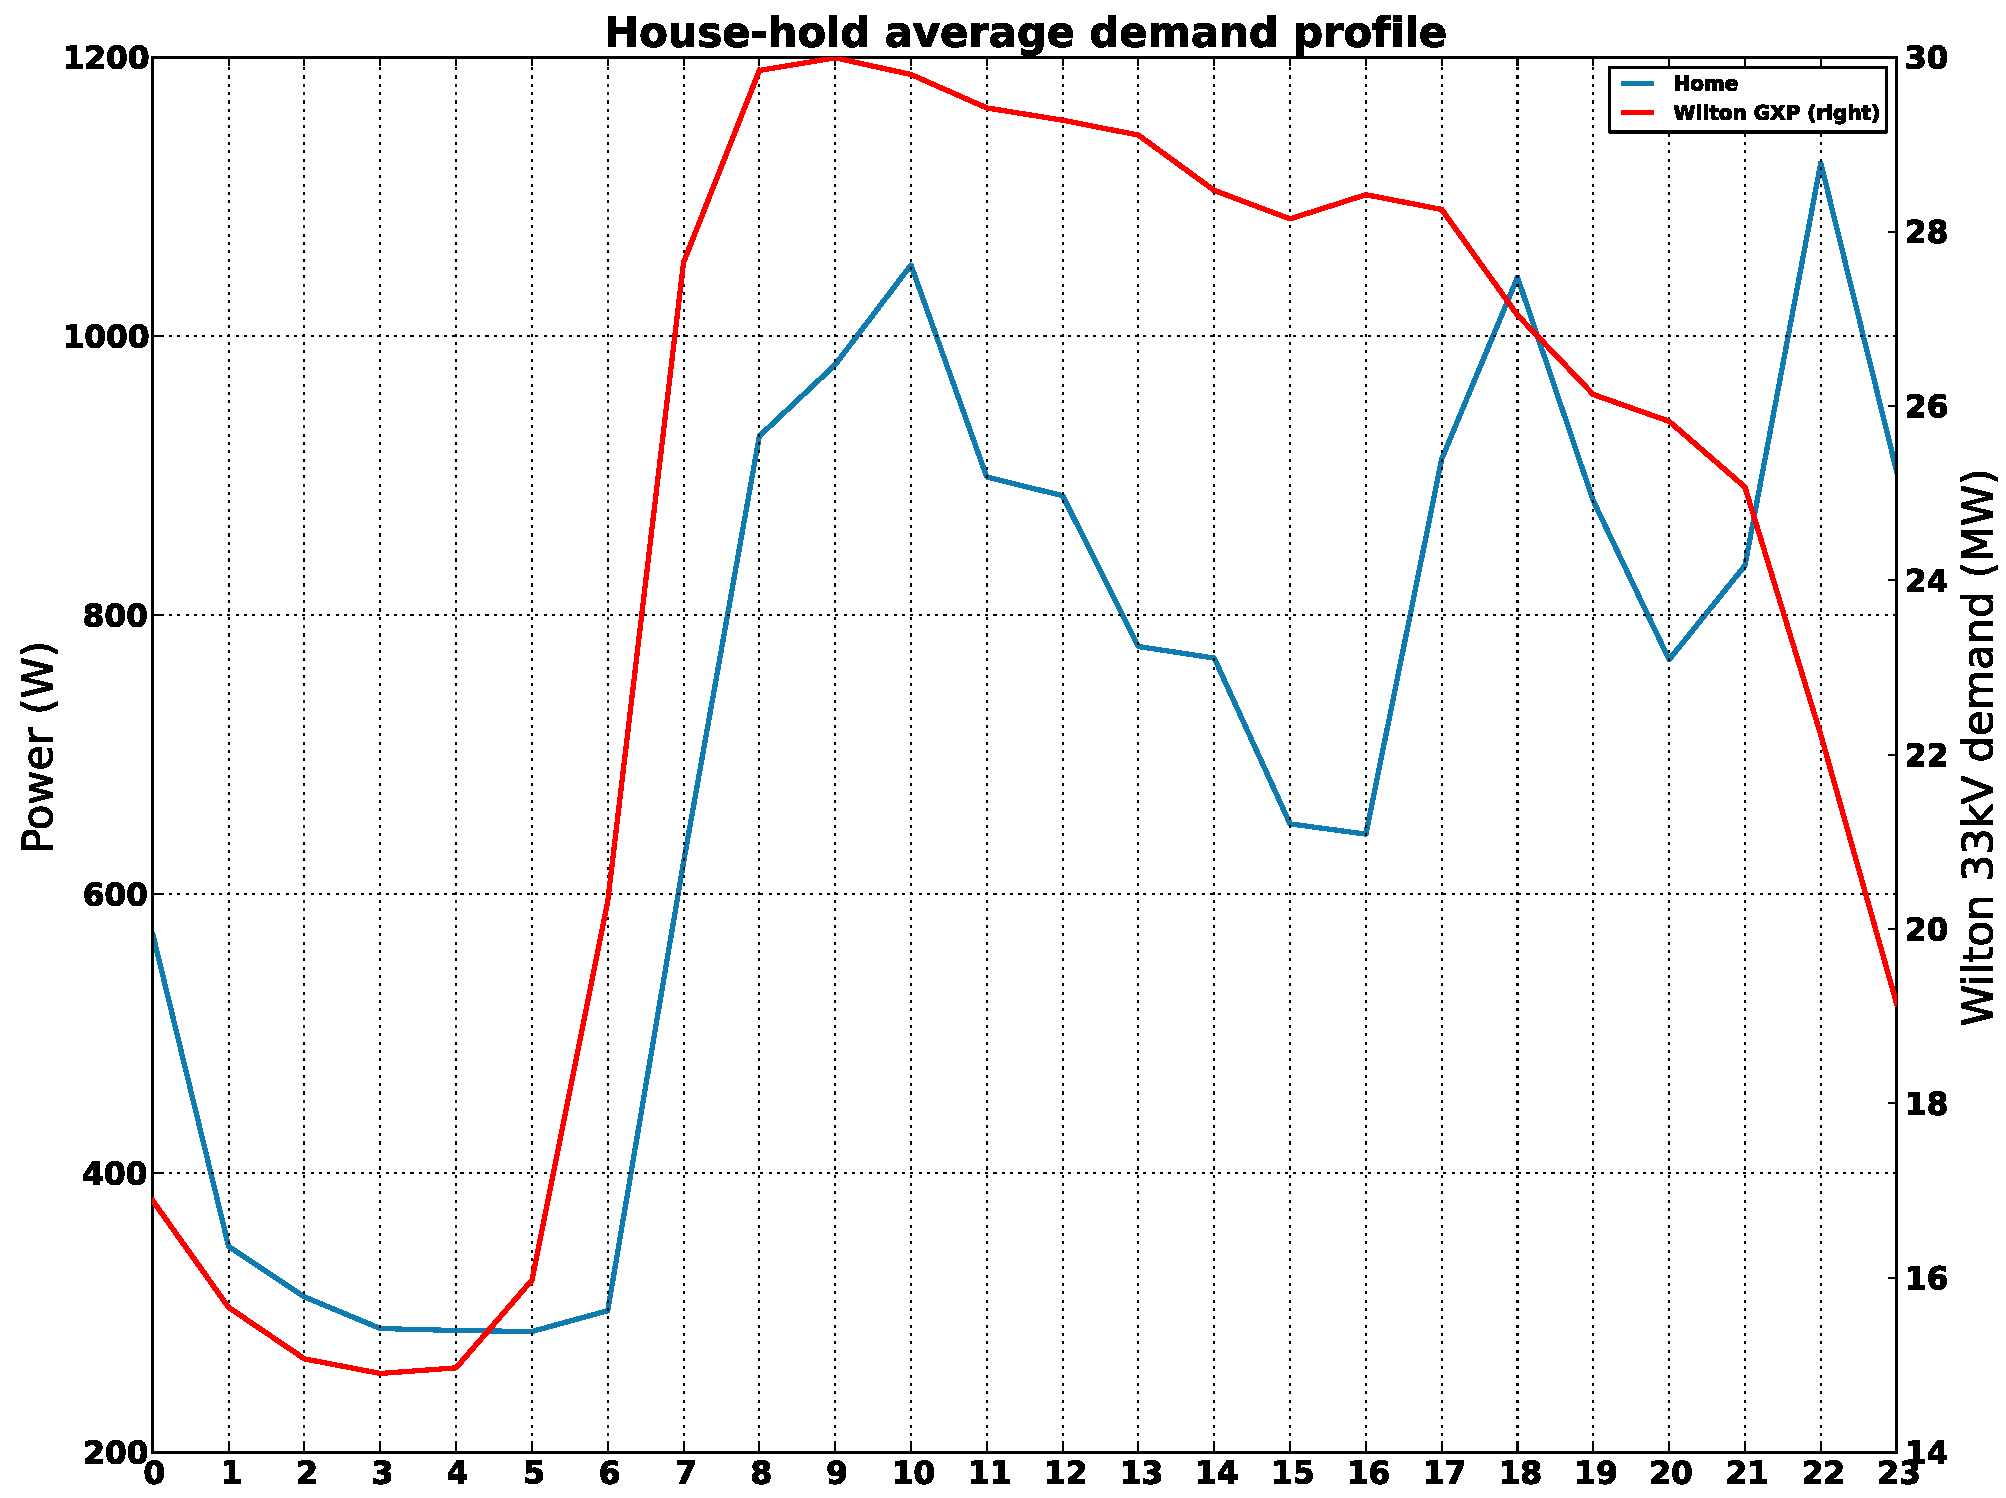
\includegraphics[width=0.875\columnwidth]{125_years_of_data_files/125_years_of_data_fig_05.pdf}
\par
\end{center}
\caption{Average daily demand profiles (between November 2012 to April, 2013) of the author's home vs Wilton GXP in Wellington.}
\label{fig:dp}
\end{figure}

%A boxplot of the hourly usage pattern is also illustrated.


\begin{figure*}[hbtm]
\begin{center}
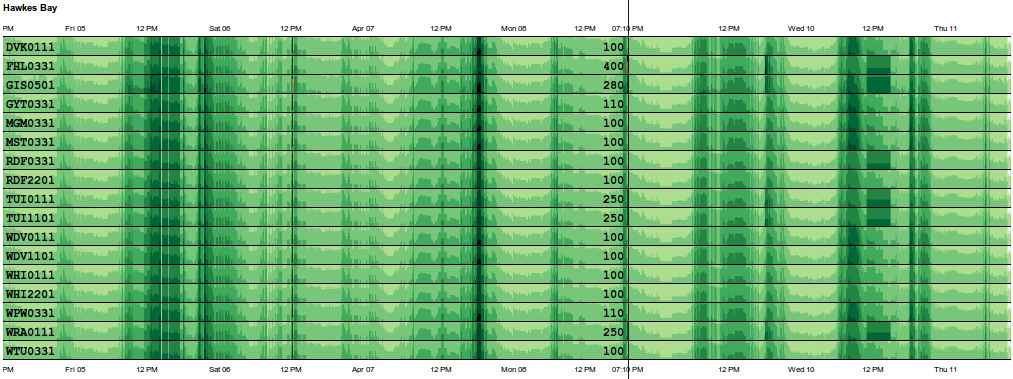
\includegraphics[width=1\textwidth]{rtpm2.png}
\end{center}
\caption{Example of visualization of spot prices using horizon charts.  Prices observed in Hawkes Bay over a week in early April, 2013.}
\label{fig:pm}
\end{figure*}

\begin{figure*}[hbtm]
\begin{center}
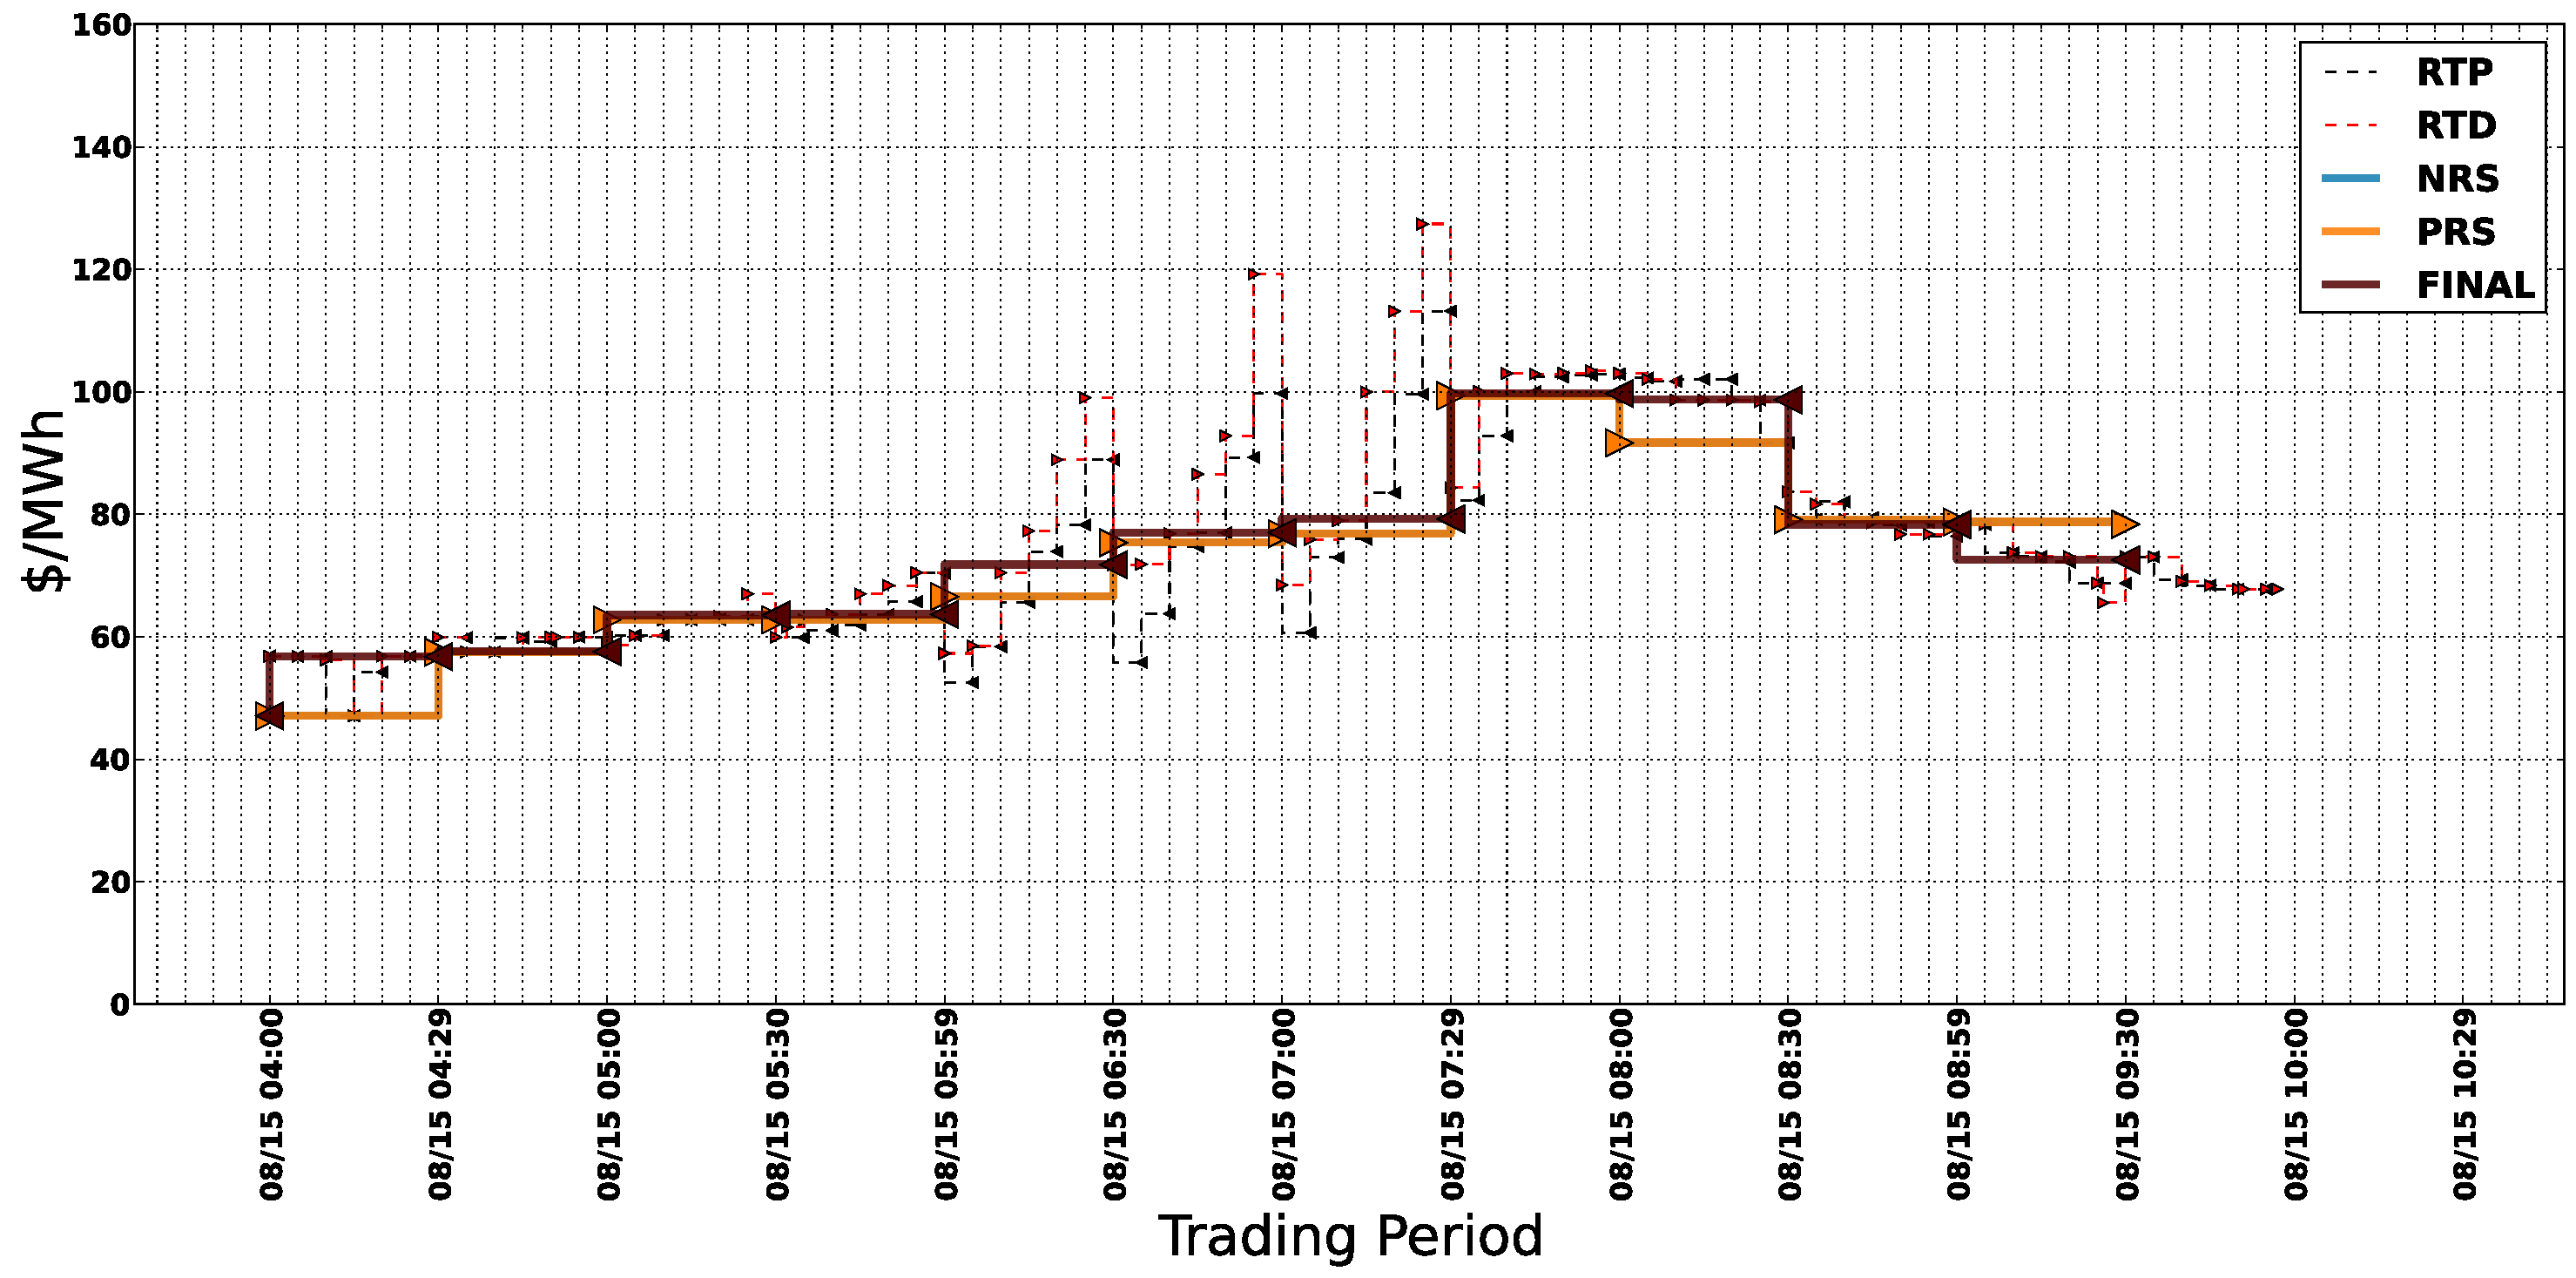
\includegraphics[width=1\textwidth]{125_years_of_data_files/125_years_of_data_fig_06.pdf}
\end{center}
\caption{Example of the difference that can be observed it different forward looking and backward looking price series in the NZ electricity market.}
\label{fig:pd}
\end{figure*}

\newpage

\section{Real-time spot market price monitoring}\label{sec:5m}
\setstretch{0.98}

The market performance team at the Electricity Authority has a role to play in monitoring the market.  As a tiny part of this, an automatic real-time price monitor system has been set up using the Python programming language.  Currently, every 5 minutes the system does the following:
\begin{enumerate}
\item FTPs the WITS FTP server and downloads the most recent 5 minute prices;
\item parses the data into memory; 
\item adds the data to an ad-hoc database; 
\item generates various statistics, including max/min gxps and average regional prices; 
\item interactively plots price trends at all GXPs for the last week using Javascript and viewed in a web-browser; 
\item sends SMS alert text messages under certain conditions.
\end{enumerate}

Figure~\ref{fig:pm} illustrates the price monitor in action, in this case prices in the Hawkes Bay region for the Week ending 11am Thursday the 11th of April, 2013 are shown. The picture uses a concept called horizon charts which are able, with the help of contrast, to plot time-series data in a confined space\footnote{This uses an open-source Javascript library called d3.js, along with a module called cubism.js developed by Mike Bostock and freely available on-line.}.  This type of visualisation is ideal for monitoring large data sets.  In the case of the NZ electricity market, all prices over the 250+ GXP's for the past week can be inspected within a matter of seconds.  The bands of decreasing contrast indicate increasing prices, until a threshold is reached where the colour switches from shades of green to red.  Here, at 7:10pm on Monday the 5th of April, prices reached around \$400/MWh at Fernhill in Hawkes Bay (FHL0331).  This was likely caused by a temporary constraint on the network in the region, perhaps in this case the interconnecting transformers at Redcliff.  On Wednesday afternoon the same transmission constraint bound resulting in high prices in the same region. 

Although only one region is illustrated, all regions are available for visualisation.

One issue with real-time prices is the differences observed between real-time and final prices.  These differences may be due to a number of factors including; inaccurate demand forecasts or bids, generator ramp rates, intermittent generation, among others.  Figure~\ref{fig:pd} illustrates a fairly typical example of the differences that can occur during a morning peak period, in this case on the 8th of August, 2013.  The Non-Responsive and Price-Responsive Schedules (NRS/PRS) indicate the final scheduled prices before the trading period started, i.e, they are forward looking or ex-ante prices.  These schedules, along with final prices (which are backward looking, ex-post) are calculated every half-hour, or trading period.  Additionally, there are two 5 minute price series.  The 5 minute ex-post ``real-time'' price series which is published every 5 minutes, and a forward looking (ex-ante) ``distpatch'' 5 minute price series that is used by the System Operator and is not published.  The dispatch is solved automatically every 5 minutes, or can be invoked by an operator at any time between. 

\section{Transmission unplanned outage data}\label{sec:fo}
As part of the CDS, Transpower provides two excel files that list, in cronological order, forced outages of Transpower's assets.  One file contains AC transmission outages, while the other contains unplanned HVDC system outages.   Each transmission forced asset outage has a unique identifier along with a code that describes the actual equipment that was removed from serive.  This is called the primary outage.  Associated with each primary outage is a list of additional secondary outages that were removed as a result of the primary outage.  This section takes a brief look at the HVAC outages on Transpowers network.  

The table below illustrates a slightly altered form of the data.

%\begin{codecell}
%\begin{codeoutput}
{\tiny
\begin{verbatim}
                               
        Ident   Flt_Item Rem_Item Start             End  \                                            
        SS99101 LIV-NSY1 LIV-NSY1 1999-07-02 11:20 1999-07-02 11:30   
                         NSY-TF-1 1999-07-02 11:20 1999-07-02 11:40   
                         NSY-TF-2 1999-07-02 11:20 1999-07-02 11:41   
                         NSY-ROX1 1999-07-02 11:20 1999-07-02 11:30   
        SS99102 CML-FKN2 CML-FKN2 1999-07-02 22:13 1999-07-02 22:36   
                         FKN-TF-4 1999-07-02 22:13 1999-07-02 22:38   
        SS99103 CML-FKN2 CML-FKN2 1999-07-02 22:50 1999-07-02 23:00   
                         FKN-TF-4 1999-07-02 22:50 1999-07-02 23:16   
        SS99104 CML-FKN1 CML-FKN1 1999-07-02 23:04 1999-07-02 23:11   
                         FKN-TF-2 1999-07-02 23:04 1999-07-02 23:12   
        SS99105 CML-FKN2 CML-FKN2 1999-07-02 23:09 1999-07-03 16:27   
                         FKN-TF-4 1999-07-02 23:09 1999-07-03 16:27   

\end{verbatim}
}
%\end{codeoutput}
%\end{codecell}
\normalsize
\setstretch{1}

where the fields are:
\begin{description}[font=\bfseries, leftmargin=0.5cm,style=nextline]
\item[Ident] Incident Identifier that links all the records associated with one fault. Note: the second letter indicates an `S' for South or `N' for North Island;
\item[Flt\_Item] The primary forced outage identifier indicating the item of equipment which caused the forced outage. There is usually one of these per incident. The exception is for a double circuit fault;
\item[Rem\_Item] The secondary outages forced out of service caused by the primary outage;
\item[Island] Indicator of where the outage occurred;
\end{description}

For example, at 11:20am on 2nd of July, 1999, the Livingston--Naseby--Roxburgh circuit tripped also taking out the supply transformers at Naseby.  Although the LIV--NSY--ROX circuit was back in service 10 minutes later, it took 20/21 minutes before the Naseby supply transformers were back in service.  

The following notes are included in the CDS. 
 
\begin{enumerate}
\item Forced Outages are those for which the equipment was tripped or manually taken out of service within 24 hours of the fault occurring or being discovered.
\item A circuit is deemed out of service if any circuit breaker is open. In some cases, a forced outage may be recorded against a circuit section rather than the whole circuit, in particular for three terminal circuits. A transformer is deemed out of service if either the HV or LV circuit breaker is open (an open CB on the tertiary winding is generally not considered to constitute a transformer outage).
\item A trip – autoreclose-trip sequence is shown as one incident (with one identifier) if the autoreclose was unsuccessful because of a persisting fault.
\item If a second fault occurs or is discovered when attempting to return equipment to service, a second incident is recorded with a second identifier, e.g. failed autoreclose because of a protection fault; or a transformer cannot be returned to service because of a CB problem.
\item A number of outages within a relatively short space of time will generally be recorded under one identifier if they all had the same cause, e.g. a tree causes three trippings within 10 minutes. If the outages are caused by separate faults they will have separate identifiers, e.g. if a circuit trips for lightning 3 times in 10 minutes.
\item Unplanned outages caused by a delayed return-to-service after planned maintenance works are not included.
\item Whilst Transpower has used reasonable endeavours to ensure that this data is accurate, there is no guarantee that it is error free.
\end{enumerate}

\begin{figure}
\begin{center}
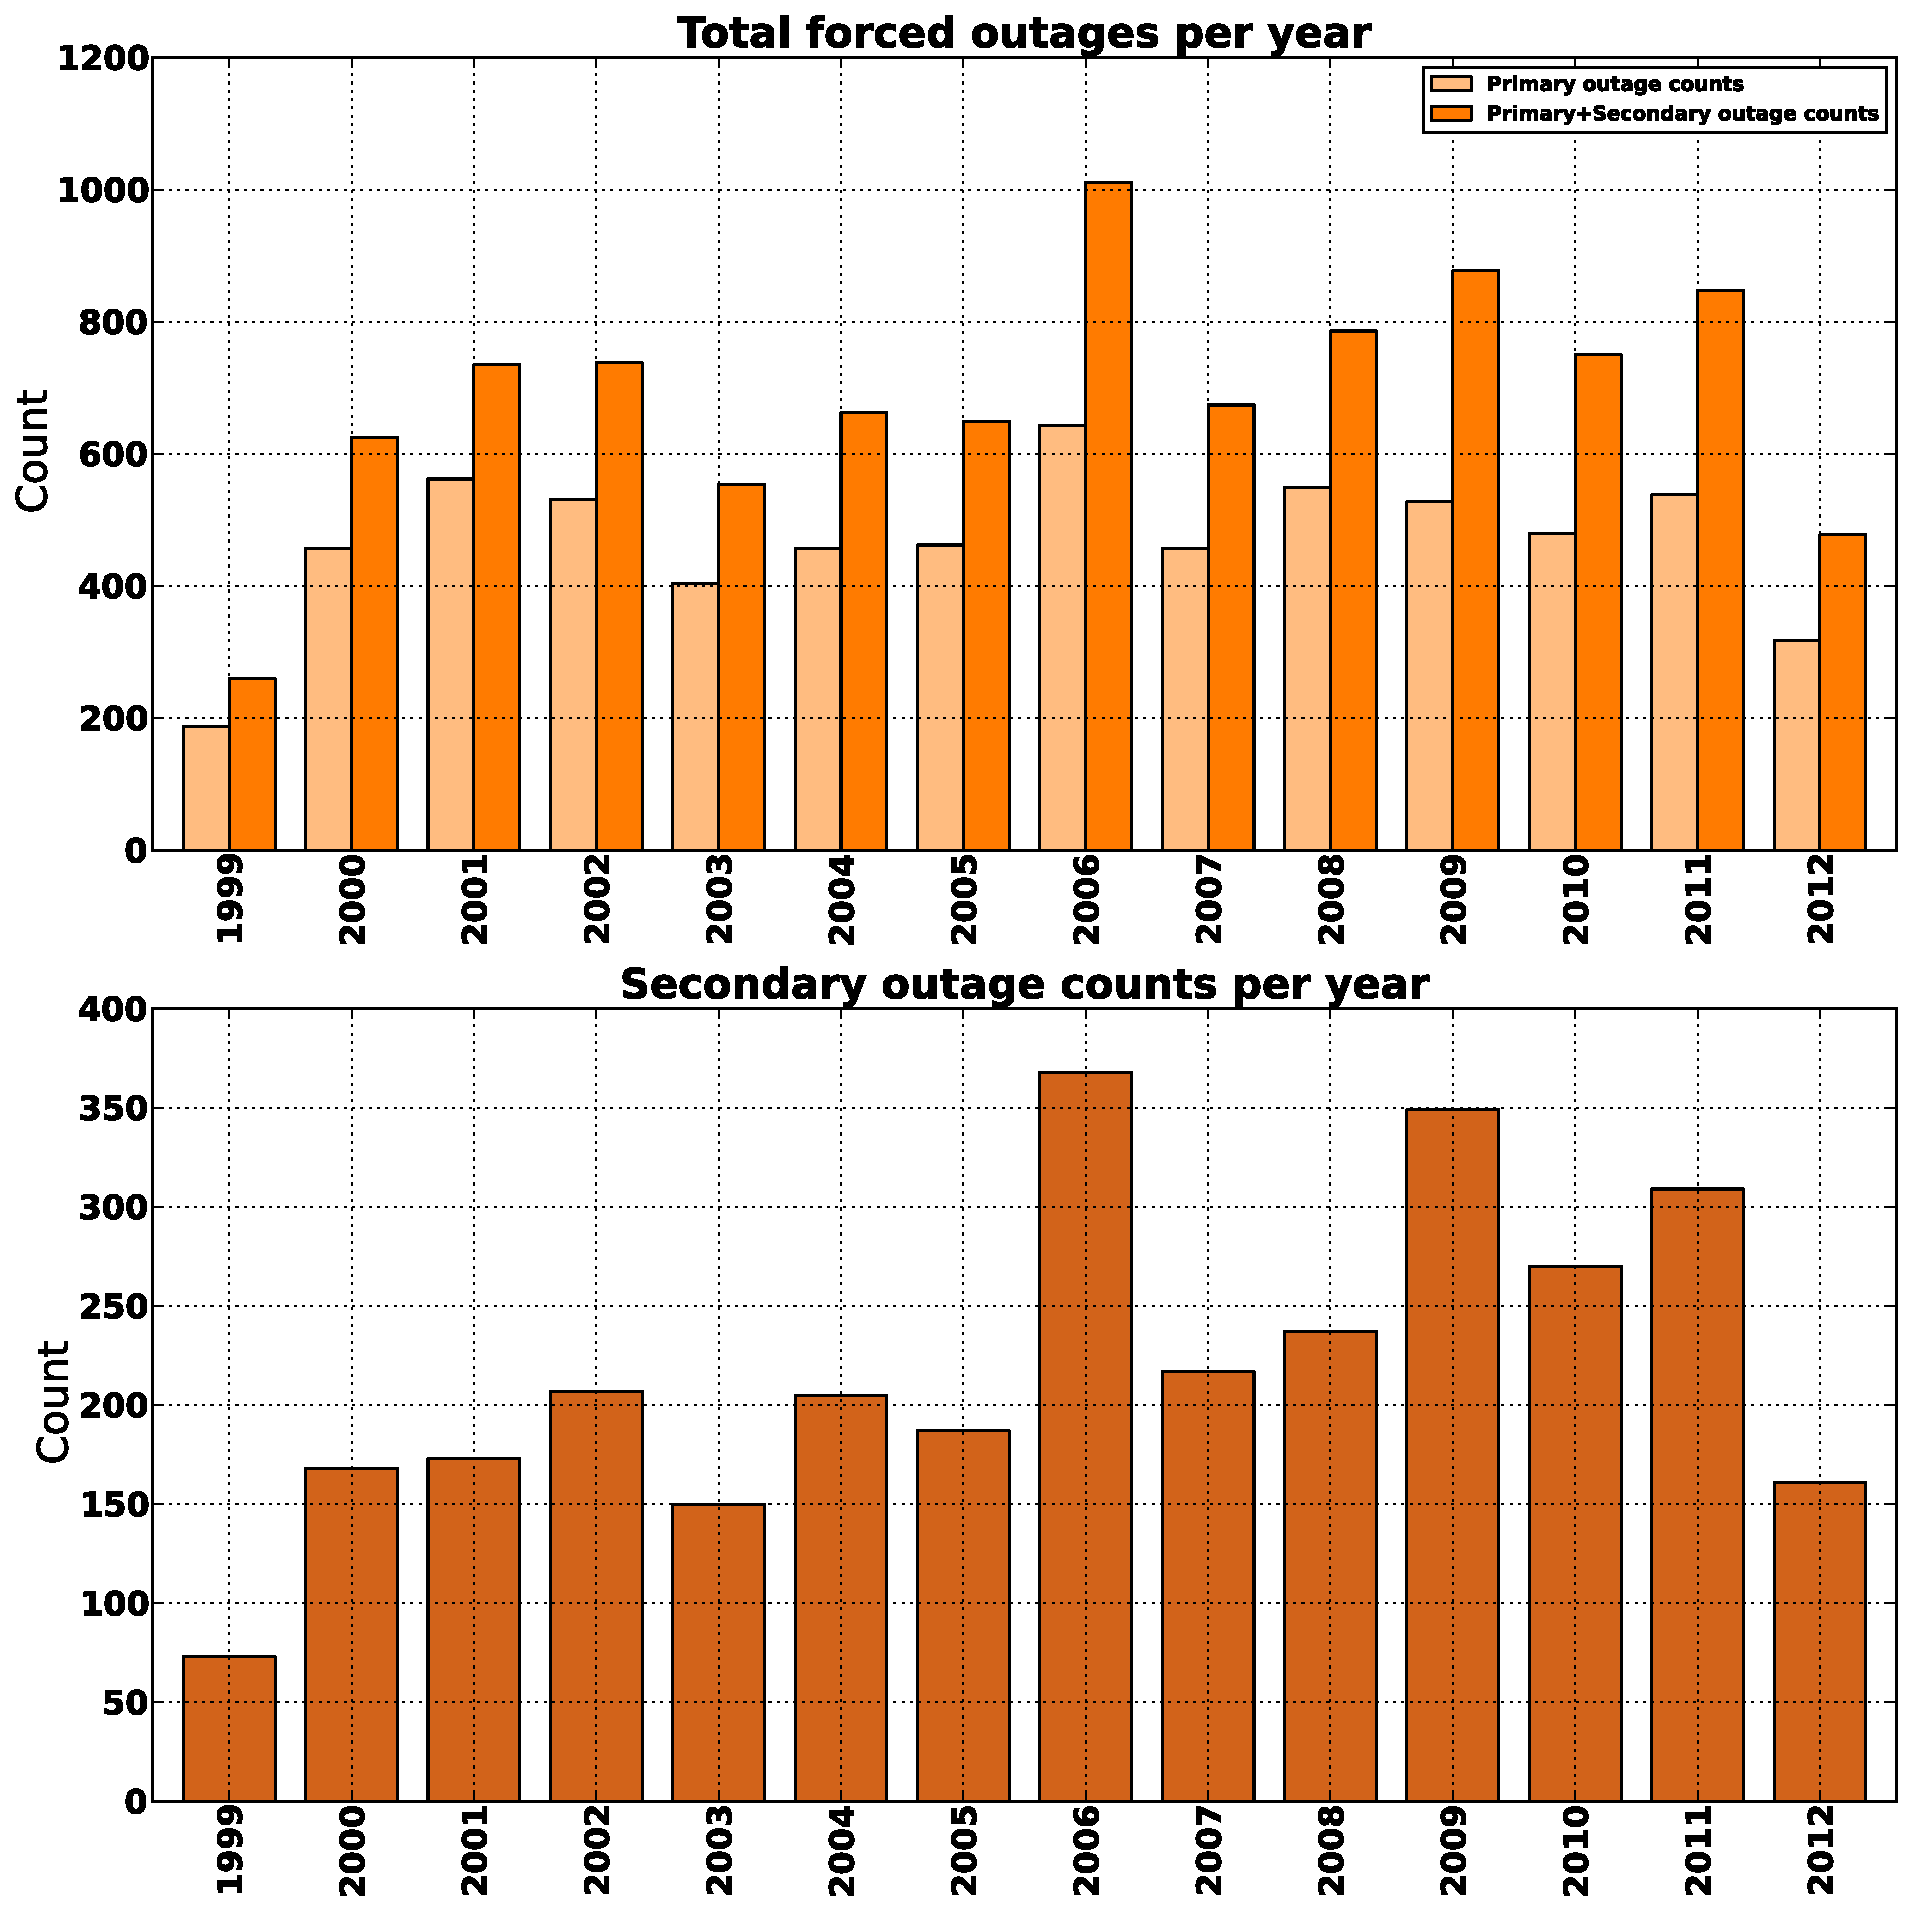
\includegraphics[width=1\columnwidth]{125_years_of_data_files/125_years_of_data_fig_07.pdf}
\par
\end{center}
\caption{Annual counts of total forced HVAC outages.}
\label{fig:ct}

\end{figure}

\begin{figure}
\begin{center}
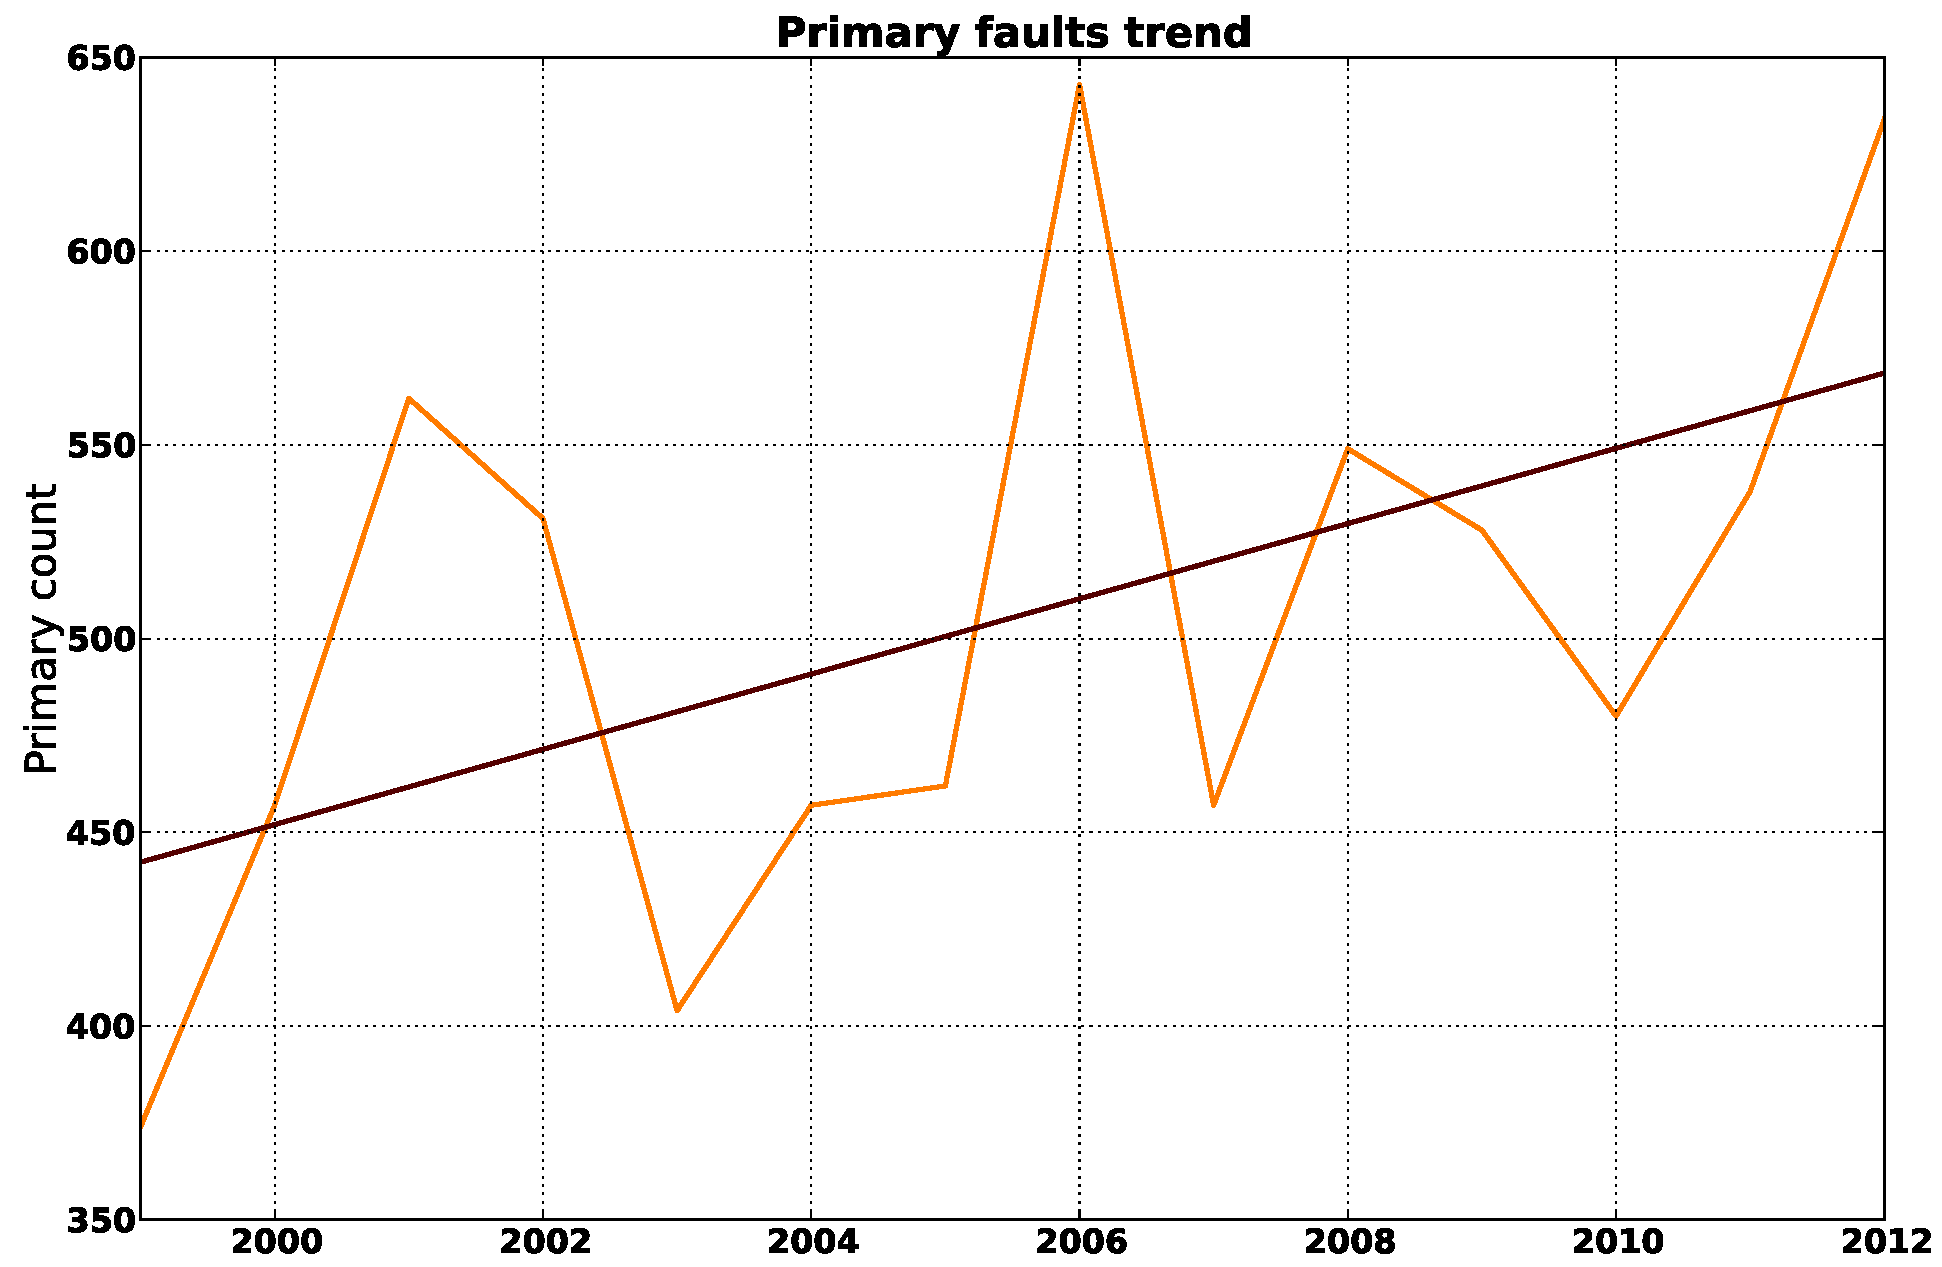
\includegraphics[width=1\columnwidth]{125_years_of_data_files/125_years_of_data_fig_08.pdf}
\end{center}
\label{fig:rg1}
\caption{A straight line fit of primary outage counts}
\end{figure}

\setstretch{0.95}

Lets take a look at the total forced outages per year\footnote{Note: 1999 and 2012, at the time of writing, had only a half-year of data.  Counts for this data are multiplied by 2 in the OLS regression analysis.}

As illustrated in Figure~\ref{fig:ct}, 2006 was a particularly bad year with a maximum of almost 650 forced outages, or, on average, one every 14 hours.  In contrast, 2003 had only 404 primary outages or, on average, one every 22 hours.  The average over the entire data series is 505 outages per year, or one every 17.3 hours.  On visual inspection there appears a concerning upward trend.  However, with such varying data it is often difficult to test this statistically.   One method is to attempt to fit a straight line.  This is achieved using an ordinary least squares, or OLS, linear regression model.  OLS models can also output various coefficients and statistical indicators, including measures such as confidence intervals.  

Testing this result statistically indicates the results are borderline conclusive and so we can't reject the null hypothesis or conclusively state that the primary forced outage rate is growing\footnote{As the p-values indicate. A p-value is always between 0 and 1.  It indicates the probability of the difference in the data being due to sampling error.  The p-value should be lower than a chosen significance level (0.05 for example) before you can reject your null hypothesis.}. 

\vspace{3mm}

\begin{codecell} 
\begin{codeoutput}
\begin{verbatim}
<class 'statsmodels.iolib.summary.Summary'>
"""
                            OLS Regression Results                            
==============================================================================
Dep. Variable:                 counts   R-squared:                       0.268
Model:                            OLS   Adj. R-squared:                  0.207
Method:                 Least Squares   F-statistic:                     4.403
Date:                Thu, 11 Apr 2013   Prob (F-statistic):             0.0577
Time:                        12:45:40   Log-Likelihood:                -78.224
No. Observations:                  14   AIC:                             160.4
Df Residuals:                      12   BIC:                             161.7
Df Model:                           1                                         
==============================================================================
                 coef    std err          t      P>|t|      [95.0% Conf. Int.]
------------------------------------------------------------------------------
const        442.3143     35.394     12.497      0.000       365.198   519.431
index          9.7099      4.628      2.098      0.058        -0.373    19.792
==============================================================================
Omnibus:                        1.625   Durbin-Watson:                   2.141
Prob(Omnibus):                  0.444   Jarque-Bera (JB):                1.281
Skew:                           0.630   Prob(JB):                        0.527
Kurtosis:                       2.220   Cond. No.                         14.7
==============================================================================
"""
\end{verbatim}
\end{codeoutput}
\end{codecell}
\setstretch{0.94}

Although the total count of primary, or causer faulted items can not be conclusively proved to be growing, the same can not be said about the increase in secondary outages associated with each primary outage (as illustrated in Figure~\ref{fig:ct}).  I.e., it appears that the size of forced outage event, in terms of how many secondary items are tripped, is increasing.  

To conclude this, we assume the annual count of secondary outages as a proxy for event size.  This seems reasonable; instead of being measured by lost electrical demand\footnote{Note: many of the forced outages will not necessary result is lost demand.}, we measure how many additional elements were lost due to the primary causing outage, i.e., the number of additional transformers, circuits or line sections lost when a primary forced outage occurs. 


\begin{figure}
\begin{center}
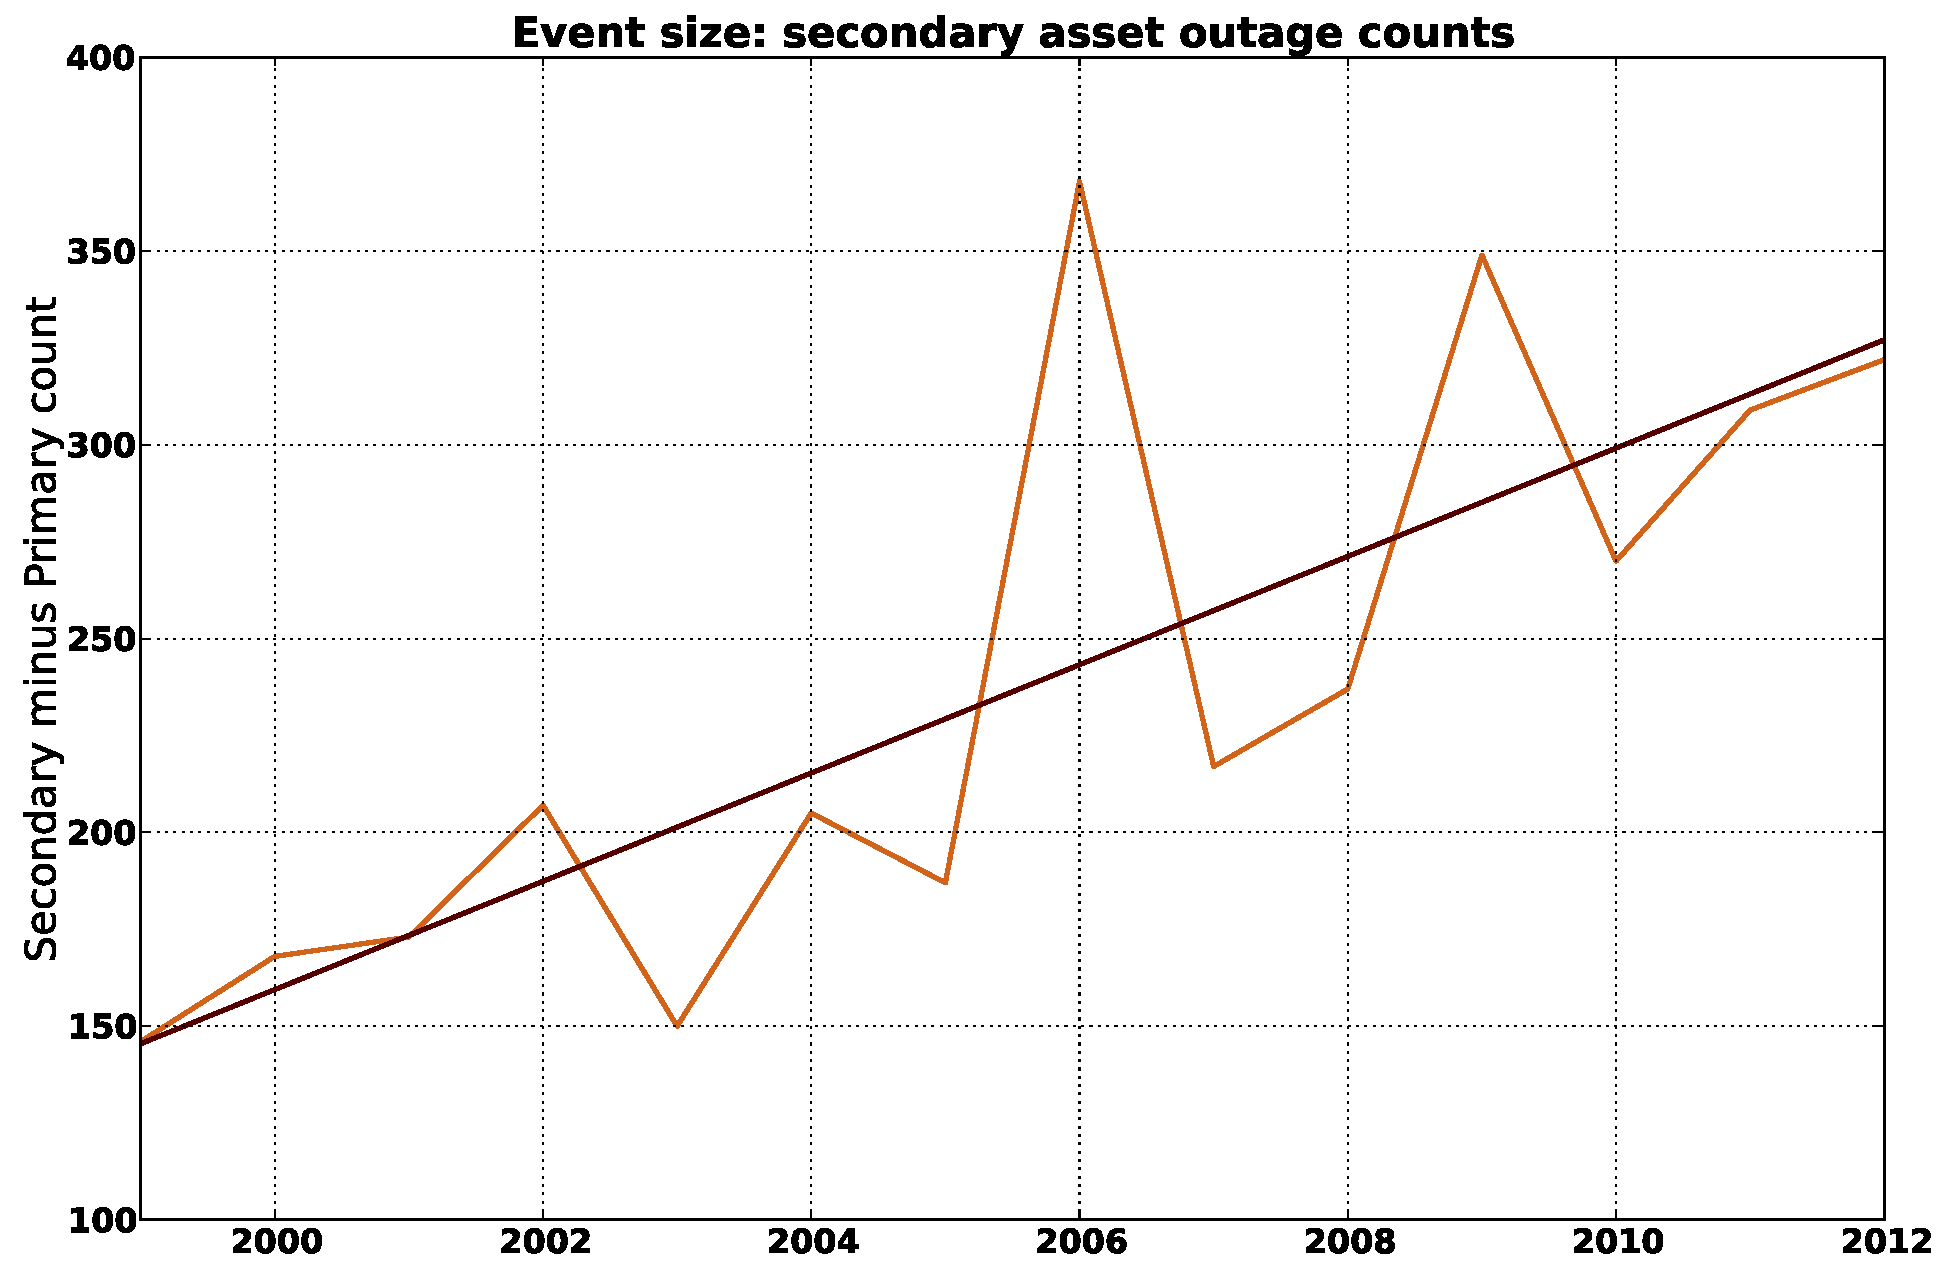
\includegraphics[width=1\columnwidth]{125_years_of_data_files/125_years_of_data_fig_09.pdf}
\par
\end{center}
\label{fig:eight}
\caption{A straight line fit of secondary outage counts.}
\end{figure}

\vspace{3mm}

\begin{codecell}
\begin{codeoutput}
\begin{verbatim}


<class 'statsmodels.iolib.summary.Summary'>
"""
                            OLS Regression Results                            
==============================================================================
Dep. Variable:                 counts   R-squared:                       0.611
Model:                            OLS   Adj. R-squared:                  0.578
Method:                 Least Squares   F-statistic:                     18.83
Date:                Tue, 09 Apr 2013   Prob (F-statistic):           0.000962
Time:                        12:01:37   Log-Likelihood:                -73.147
No. Observations:                  14   AIC:                             150.3
Df Residuals:                      12   BIC:                             151.6
Df Model:                           1                                         
==============================================================================
                 coef    std err          t      P>|t|      [95.0% Conf. Int.]
------------------------------------------------------------------------------
const        145.4571     24.628      5.906      0.000        91.798   199.117
index         13.9736      3.220      4.340      0.001         6.958    20.989
==============================================================================
Omnibus:                       11.111   Durbin-Watson:                   2.908
Prob(Omnibus):                  0.004   Jarque-Bera (JB):                6.867
Skew:                           1.466   Prob(JB):                       0.0323
Kurtosis:                       4.782   Cond. No.                         14.7
==============================================================================
"""
\end{verbatim}
\end{codeoutput}
\end{codecell}

Figure~\ref{fig:ct} and the table below illustrate the results of the OLS regression analysis.   This suggests, with reasonable certainty, that the size of event outages, in terms of the amount of secondary items effected, has been growing.  

The 95\% confidence interval is between 7 and 21 additional outages per year with an average rate of growth of around 14 additional secondary outages per year, for each year, over the past 13 years. 

Assuming the data is to be believed, there could be many reasons for this increasing trend, including: 
    
\begin{itemize}
\item increased system size;
\item increased peak demand;
\item increased complexity (protection systems and settings?)
\item increased human error; 
\item data/communication issues?
\item actual reported dataset issues?
\item lack of maintenance; 
\item lack of co-ordination in planned outages? 
\end{itemize}

This section has illustrated the results of an analysis on the forced outage data that is openly published as part of the Centralised Data Set (CDS).  It suggests that primary forced outages may be on the increase, although this is borderline statistically.  It does however appear that the size of forced outages, in terms of the number of secondary outages resulting from an initial primary outage, is on the increase, at least over the last 13 years. 

Many more analyses have and can be made on this dataset.  For example, grouping the data at the island level can give island wide information and we can also identify those assets who trip most often, etc.  If interested, contact the author for more information or for a copy of the IPython Notebook, and data files used in this analysis.

\section{POCP data}\label{sec:po}

The Planned Outage Co-ordination Process (POCP) and the POCP database are run by the System Operator and provide a voluntary platform through which industry participants can publish, or broadcast, their intended planned generation and transmission outages.

The current system was jointly developed by participants, including Transpower, through a series of joint industry workshops during 2002/2003.  The WAG/System Operator are currently reviewing the POCP process.

The data, although available to participants, is not openly available, requiring registration and a password.  The POCP database is available at: 
    
\url{http://www.pocp.redspider.co.nz/} with a dashboard available at:
\url{http://nzeb.redspider.co.nz/}\footnote{A guide is also avialable at: \url{http://pocp.redspider.co.nz/doc/guide.php}}
        
Under the POCP:
\begin{itemize}
\item Asset owners provide information about their planned outages;
\item The System Operator assesses any potential conflict with its Principle Performance Objectives, based on the information provided, and publishes the results of the assessment;
\item Any interested party may view both the planned outage data, and the results of the System Operator assessments, so that they are aware of planned outages that may require their consideration or action;
\item The POCP database supports the POCP by receiving, collating and publishing the planned outage data from asset owners, and is also used to publish the results of the System Operator assessments.
\end{itemize}

The System Operator provides a very nice dashboard through \url{http://nzeb.redspider.co.nz/} which provides a more graphical interface with custom alerts etc.  This is great for future planning, and outage assessment, as required by the System Operator, but as it turns out, not so great for inspecting historic outages.   The Market Performance team at the Authority are interested in both forward looking and historic outages.   There are several issues with the way the current POCP database is setup:  
\begin{description}[font=\bfseries, leftmargin=0.5cm,style=nextline]
\item[Generators often cancel an outage after the outage window has finished]  This makes if difficult to tell, retrospectively, weather an outage actually happened at all.  A way around this is to inspect the Last Modified field and make the assumption that as the outage was modified after the ``End time'' field, the outage did in fact occur.  This is not ideal.  Ideally, outages should never be cancelled if they occurred.  Outage's should only be cancelled if they do not occur. If an outage ends early, then the End Time can be modified to reflect this.  
\item[Inconsistent data]  The current database allows generators quite a lot of freedom when entering data.  This is problematic and makes analysis of the data very difficult.  For example;
        \begin{itemize}
        \item One generators generation outages are never confirmed.  They are all marked as Tentative!;
        \item Outages can be entered multiple times with different identifiers and start/end dates;
        \item Outages are sometimes entered with the  ``MW loss'' field blank;
        \item As generators can choose an outage ID, over the history of the dataset, there are Outages whose IDs are not unique.
        \end{itemize}
\end{description}
Despite these moans, the data can be made semi-useful by investigating the outages as they occur in time.  This is achieved by time-serializing the data and constructing a time series of outage MW magnitude.  To get around some of the issues discussed above, some ad-hoc time dependent logic is applied, in particular to determine if a cancelled outage did in fact occur.  

An output of this time-serialisation process is illustrated in Figure~\ref{fig:pocp}.  This is an interactive data visualisation that is able to list the outages that have occurred, or are likely to occur, by selecting a sample date range with a mouse-click-drag.  To achieve this, a Python script is used to download the database and manipulate the data into a required form, including the construction of the time series data.  A local webserver is then set-up to plot the data using, in this case, the excellent Javascript d3 library combined with a d3 module called "cross-filter".

\begin{figure}[hbtm]
\begin{center}
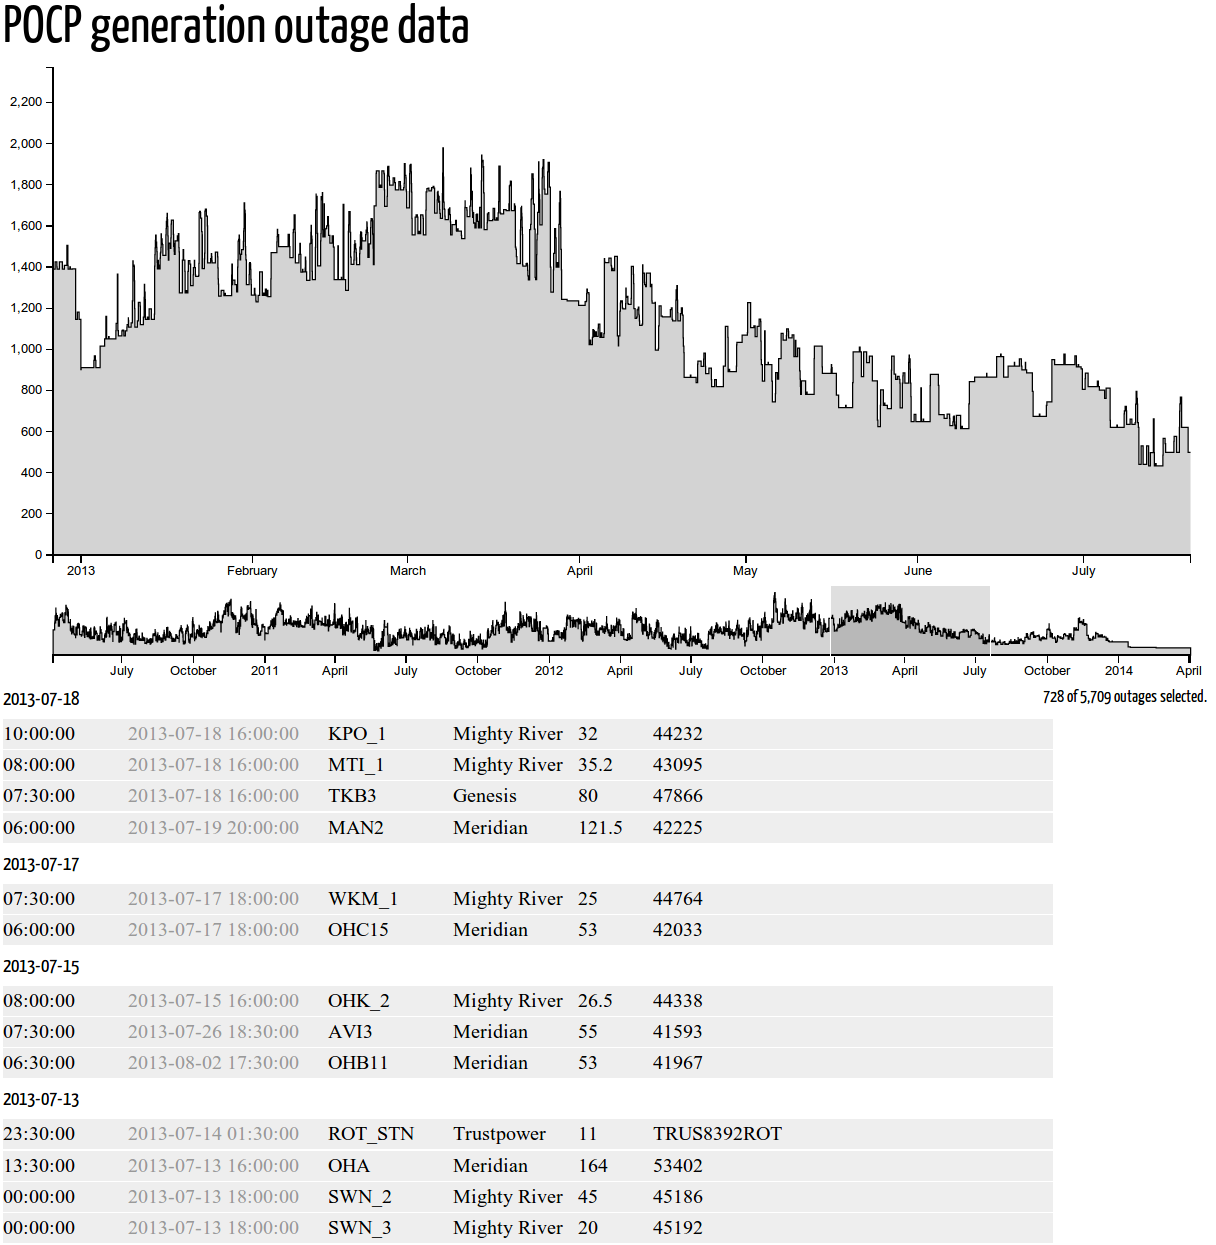
\includegraphics[width=1\columnwidth]{pocp2.png}
\end{center}
\caption{Example of POCP monitoring}
\label{fig:pocp}
\end{figure}


\section{Open source software}\label{sec:os}

The development of quality open source software has taken off in recent years due mainly to the ease of software colabaration through the use of the Git version control software and Github.

This paper is writen entirely with open-source, freely availble software.   All data analysis, outputs and in fact the entire text of this paper have been written within a single iPython notebook.  
The iPython notebook allows an interactive python code devleopment environment from within the web-browser.  The Notebook and packages such as Numpy and Pandas have been the authors daily tools now for over 18 months, replacing both Matlab, Excel and R.

The use of client-side (browser based) visualisation for interactivity is also growing extremely quickly.  Javascript/d3 and it's various modules appear to be leading the pack.

\section{Summary}

In an industry flush with data, data analysis and visualisation are becoming increasingly important.  The expoential growth in electrical generation in the first half of the 20th centry has in certain ways been replaced by an exponential growth in data.  A single hour of data logging from a single home energy monitoring system will contain more data than the total historical generator name-plate data series used in this paper.  For the engineering/data analyst, it is easy to become engulfed with too much data.  Tools (and knowing how to use them efficiently) are important.  In recent years the rise of powerful open-source software has in ways overtaken many commercial products.  In particular, the Python programming language combined with the iPython notebook make for a formidable interactive workspace, ideal for both data analysis and visualisation.  


\begin{thebibliography}{1}

\bibitem{wes}
\emph{Python for Data Analysis},\hskip 1em plus
  0.5em minus 0.4em\relax O’Reilly Media, Inc.
, Wes McKinney, 2013.
\bibitem{scott}
\emph{Interactive Data Visualization for the web},\hskip 1em plus
0.5em minus 0.4em\relax O’Reilly Media, Inc.
, Scott Murry, 2013.
\bibitem{git}
\emph{Version control with GIT},\hskip 1em plus
0.5em minus 0.4em\relax O’Reilly Media, Inc.
, 2nd. Ed, Jon Loeliger and Mattew McCullough, 2012.
\bibitem{js}
\emph{JavaScript Enlightenment},\hskip 1em plus
0.5em minus 0.4em\relax O’Reilly Media, Inc.
, Cody Lindley, 2013.
\bibitem{bul}
\scriptsize
\url{http://www.doc.govt.nz/Documents/science-and-technical/sap237.pdf}
\footnotesize
\bibitem{rf1}
\scriptsize
\url{http://www.reefcottage.co.nz/41_history.htm}
\footnotesize

\bibitem{rf2}
\scriptsize
\url{http://www.reeftongold.co.nz/morning-heritage-tours/electric-light}
\footnotesize

\bibitem{rf3}
\scriptsize
\url{http://www.TeAra.govt.nz/en/gold-and-gold-mining/12/2}
\footnotesize
\bibitem{gh}
\scriptsize
\url{https://github.com}
\footnotesize
\bibitem{ipy}
\scriptsize

\url{http://ipython.org/}

\end{thebibliography}

\emph{\ldots On Wednesday the 24'th of November 1886, bright light had been brought to the bars of Dawson's, Kater's, Stevenson's and William's hotels by showman Walter Prince via underground cable through attaching a one kilowatt generator to the Oxley's brewery's steam engine. The test required regular visits of the spectators between the hotel and the brewery, and there was high demand at each point of supply. As a result, many were carrying an overload and it was not only the hotel that was lit up.\ldots''}



\end{document}
